\documentclass[12pt,a4paper]{article}
\usepackage[a4paper, margin=0.8in, headheight=14pt]{geometry}
\usepackage{fontspec}
\usepackage{unicode-math}
\setmainfont{TeX Gyre Pagella}
\setmonofont[Scale=0.88]{TeX Gyre Cursor}
\setmathfont{Latin Modern Math}
\usepackage{xcolor}
\usepackage{colortbl}
\usepackage{titlesec}
\usepackage{enumitem}
\usepackage{tabularx}
\usepackage{booktabs}
\usepackage{array}
\usepackage{amsmath}
\usepackage{tikz}
\usetikzlibrary{shapes.geometric, arrows.meta, positioning, calc, fit, decorations.pathreplacing, decorations.pathmorphing, patterns}
\usepackage[american]{circuitikz}
\usepackage{tcolorbox}
\tcbuselibrary{skins, breakable}
\usepackage{hyperref}
\usepackage{fancyhdr}
\usepackage{graphicx}
\usepackage{microtype}
\hyphenpenalty=10000
\exhyphenpenalty=10000
\sloppy
\usepackage{caption}
\usepackage{setspace}
\usepackage{multirow}
\usepackage{tocloft}
\newcommand{\Q}[1]{\textbf{#1}\par\noindent\ignorespaces}
\definecolor{myred}{RGB}{196,30,58}
\definecolor{mydark}{RGB}{30,30,50}
\definecolor{mygreen}{RGB}{14,120,80}
\definecolor{myteal}{RGB}{0,130,140}
\definecolor{myamber}{RGB}{180,100,0}
\definecolor{mypurple}{RGB}{100,30,160}
\definecolor{mygray}{RGB}{246,247,249}
\definecolor{mgframe}{RGB}{180,185,200}
\definecolor{watermark}{RGB}{145,150,170}
\definecolor{hdrred}{RGB}{250,232,235}
\definecolor{hdrgreen}{RGB}{220,244,233}
\definecolor{hdrteal}{RGB}{220,242,244}
\definecolor{hdramber}{RGB}{253,242,215}
\definecolor{hdrpurple}{RGB}{238,228,255}
\definecolor{hdrgray}{RGB}{238,240,245}
\definecolor{rowalt}{RGB}{250,251,253}

\titleformat{\section}{\large\bfseries\color{myred}}{\thesection.}{0.5em}{}[\vspace{1pt}{\color{myred}\rule{\linewidth}{0.8pt}}]
\titleformat{\subsection}{\normalsize\bfseries\color{myteal}}{\thesubsection}{0.5em}{}
\titlespacing*{\section}{0pt}{18pt}{7pt}
\titlespacing*{\subsection}{0pt}{11pt}{4pt}
\setlength{\parindent}{0pt}
\setlength{\parskip}{4pt}
\renewcommand{\cfttoctitlefont}{\large\bfseries\color{myred}}
\renewcommand{\cftaftertoctitle}{\par\noindent{\color{myred}\rule{\linewidth}{0.8pt}}}
\setlength{\cftbeforetoctitleskip}{0pt}
\setlength{\cftaftertoctitleskip}{6pt}
\renewcommand{\cftsecfont}{\normalsize\bfseries\color{mydark}}
\renewcommand{\cftsecpagefont}{\normalsize\bfseries\color{mydark}}
\renewcommand{\cftsecleader}{\cftdotfill{\cftdotsep}}
\setlength{\cftbeforesecskip}{7pt}
\renewcommand{\cftsubsecfont}{\small\color{mydark}}
\renewcommand{\cftsubsecpagefont}{\small\color{mydark}}
\setlength{\cftbeforesubsecskip}{3pt}
\setlength{\cftsubsecindent}{1.4em}
\renewcommand{\cftpartfont}{\normalsize\bfseries\color{myteal}}
\renewcommand{\cftpartpagefont}{\normalsize\bfseries\color{myteal}}
\setlength{\cftbeforepartskip}{14pt}
\renewcommand{\arraystretch}{1.45}
\setlength{\tabcolsep}{6pt}
\arrayrulecolor{mydark}
\newcolumntype{B}[1]{>{\small\bfseries\raggedright\arraybackslash}m{#1}}
\newcolumntype{C}[1]{>{\centering\arraybackslash}m{#1}}
\newcolumntype{Y}{>{\small\raggedright\arraybackslash}X}
\renewcommand{\tabularxcolumn}[1]{m{#1}}
\newcommand{\currmodule}{Module 1}
\pagestyle{fancy}
\fancyhf{}
\fancyhead[L]{\small\color{myred}\textbf{OE-EC803A}\;\color{mydark}--- Internet of Things}
\fancyhead[R]{\small\color{myteal}\textbf{\currmodule\ Notes}}
\fancyfoot[C]{\small\color{mydark}\thepage}
\fancyfoot[R]{\small\color{watermark}\textit{\copyright\ Biraj}}
\renewcommand{\headrulewidth}{0.5pt}
\renewcommand{\footrulewidth}{0.3pt}

\hypersetup{colorlinks=true, linkcolor=myteal, urlcolor=myteal,
  pdfauthor={Biraj Sarkar},
  pdftitle={OE-EC803A --- Combined Notes}}

\tcbset{
  tikzbox/.style={colback=mygray, colframe=mgframe, boxrule=0.6pt, arc=4pt,
    left=8pt, right=8pt, top=6pt, bottom=6pt,
    colbacktitle=mgframe, coltitle=mydark, fonttitle=\small\bfseries},
  defbox/.style={colback=hdrgreen, colframe=mygreen, boxrule=0.8pt, arc=4pt,
    left=9pt, right=9pt, top=6pt, bottom=6pt,
    colbacktitle=mygreen, coltitle=white, fonttitle=\small\bfseries},
  formulabox/.style={colback=hdrteal, colframe=myteal, boxrule=0.8pt, arc=4pt,
    left=9pt, right=9pt, top=7pt, bottom=7pt,
    colbacktitle=myteal, coltitle=white, fonttitle=\small\bfseries},
  examplebox/.style={colback=hdramber, colframe=myamber, boxrule=0.8pt, arc=4pt,
    left=9pt, right=9pt, top=6pt, bottom=6pt,
    colbacktitle=myamber, coltitle=white, fonttitle=\small\bfseries},
  masonbox/.style={colback=hdrpurple, colframe=mypurple, boxrule=0.8pt, arc=4pt,
    left=9pt, right=9pt, top=6pt, bottom=6pt,
    colbacktitle=mypurple, coltitle=white, fonttitle=\small\bfseries},
  exambox/.style={colback=hdrpurple, colframe=mypurple, boxrule=1pt, arc=5pt,
    left=10pt, right=10pt, top=8pt, bottom=8pt,
    colbacktitle=mypurple, coltitle=white, fonttitle=\bfseries,
    breakable, title after break={\textbf{Frequently Asked / Viva Questions (contd.)}}}
}
\tcbset{breakable}
\tcbset{after={\color{black}}}

\tikzset{
  block/.style={rectangle, draw=myteal, fill=hdrteal,
    text width=2.5cm, align=center, minimum height=1.0cm,
    font=\small, rounded corners=3pt, line width=0.7pt},
  redblock/.style={rectangle, draw=myred, fill=hdrred,
    text width=2.5cm, align=center, minimum height=1.0cm,
    font=\small, rounded corners=3pt, line width=0.7pt},
  arrow/.style={-Stealth, thick, color=mydark},
  line/.style={draw, thick, color=mydark}
}

\newcommand{\modulestart}[2]{%
  \clearpage
  \renewcommand{\currmodule}{Module #1}%
  \renewcommand{\theHsection}{mod#1.\arabic{section}}%
  \renewcommand{\theHsubsection}{\theHsection.\arabic{subsection}}%
  \renewcommand{\theHsubsubsection}{\theHsubsection.\arabic{subsubsection}}%
  \phantomsection
  \addcontentsline{toc}{part}{Module #1: #2}%
  \setcounter{section}{0}%
  \begin{center}
    \vspace*{1.0cm}
    {\Huge\bfseries\color{myred} Module #1}\\[10pt]
    {\Large\bfseries\color{mydark} #2}\\[10pt]
    {\color{myred}\rule{0.55\linewidth}{1.2pt}}
  \end{center}
  \vspace{14pt}
}
\begin{document}

\thispagestyle{empty}

% ─── Page Border (TikZ Overlay) ────────────────────────────────────────────────
\begin{tikzpicture}[remember picture, overlay]
  % Outer border (fine line in mgframe)
  \draw[color=mgframe, line width=1.5pt] 
    ($(current page.north west) + (0.6in, -0.6in)$) rectangle 
    ($(current page.south east) + (-0.6in, 0.6in)$);
  % Inner border (finer accent line in myred)
  \draw[color=myred, line width=0.8pt] 
    ($(current page.north west) + (0.65in, -0.65in)$) rectangle 
    ($(current page.south east) + (-0.65in, 0.65in)$);
\end{tikzpicture}

\vspace*{1.0cm}
\begin{center}
  {\Huge\bfseries\color{myred} OE-EC803A}\\[10pt]
  {\LARGE\bfseries\color{mydark} Internet of Things}\\[20pt]
  {\color{myred}\rule{0.7\linewidth}{1.5pt}}\\[18pt]
  {\Large\color{myteal}\textbf{Combined Module Notes}}\\[8pt]
  {\large\color{mydark} Modules 1 -- 6}\\[40pt]
  {\normalsize\color{mydark} Semester VIII \quad$\bullet$\quad ECE \quad$\bullet$\quad 3 Credits}\\[12pt]
  {\normalsize\color{mydark} CGEC \;$|$\; B.Tech ECE (2023--27)}
\end{center}
\vspace{1.0cm}
\begin{center}
  \begin{tcolorbox}[colback=mygray, colframe=mgframe, boxrule=0.5pt, arc=3pt, width=0.85\linewidth]
    \centering\small\color{mydark}
    \textbf{Disclaimer / Study Guide Notice:}\\
    These are condensed \textbf{Short Notes} focusing on core theory, key formulas, block/circuit diagrams, and standard viva Q\&As for university exam revision. Exhaustive numerical practice problems and derivation edge cases are not covered. This serves as a quick-revision reference guide for students.
  \end{tcolorbox}
\end{center}
\vfill
\vspace{0.6cm}
\begin{center}
  {\large\bfseries\color{mypurple} Biraj Sarkar}\\[16pt]
  {\footnotesize\color{watermark}\textbf{IN ASSOCIATION WITH}}\\[8pt]
  {\small\bfseries\color{mydark} MAKAUT Wingman \quad$\bullet$\quad MAKAUT Future Minds}\\[12pt]
  {\large\bfseries\color{myteal} Cooch Behar Government Engineering College}
\end{center}
\vfill
\begin{center}{\small\color{watermark}\textit{Exam-Ready Notes}}\end{center}
\clearpage

\hypersetup{linkcolor=mydark}
\tableofcontents
\hypersetup{linkcolor=myteal}
\clearpage

% -- Module 1 -----------------------------------------------------------------
\modulestart{1}{The Internet of Things: An Overview}

\section{The Internet of Things: An Overview}
% ===============================================================================

\begin{tcolorbox}[defbox, title={Internet of Things (IoT)}]
  \textbf{The Internet of Things (IoT)} is a global network of physically interconnected objects (or ``things'') embedded with sensors, software, actuators, and network connectivity, enabling them to collect, exchange, and act on data without requiring direct human-to-human or human-to-computer interaction.
\end{tcolorbox}

\subsection{The Flavour of the Internet of Things}
IoT bridges the gap between the physical and digital worlds by introducing \textbf{digital identity} and \textbf{intelligence} to everyday objects.
\begin{itemize}[leftmargin=*, itemsep=3pt]
  \item \textbf{Physical-Digital Convergence:} Traditional devices (like a toaster or street light) are passive. IoT transforms them into active entities that communicate status and receive remote commands.
  \item \textbf{M2M (Machine-to-Machine) vs. IoT:} While M2M refers to point-to-point communication between hardware devices over dedicated lines (often isolated), IoT represents IP-based communication connecting billions of heterogeneous devices globally through standard internet protocols.
\end{itemize}

\par\vspace{6pt}\noindent
{\renewcommand{\arraystretch}{1.35}%
\begin{tabularx}{\linewidth}{|B{3.2cm}|Y|Y|}
\hline
\textbf{Parameter} & \textbf{Traditional Embedded System} & \textbf{Internet of Things (IoT)} \\
\hline
Connectivity & None or local point-to-point (isolated). & IP-based internet connection (global routing). \\
\hline
Data Processing & Local execution on microcontroller. & Distributed processing (Edge + Cloud computing). \\
\hline
Human Interaction & Direct interface (buttons, LCD screen). & Ambient, screenless, or remote app interaction. \\
\hline
Scale & Standalone, singular execution. & Interconnected, heterogeneous device fleets. \\
\hline
\end{tabularx}}

\subsection{The Technology of the Internet of Things}
The IoT system is built upon a multi-tier architectural stack:
\begin{enumerate}[leftmargin=*, itemsep=3pt]
  \item \textbf{Edge Layer (Physical/Perception):} Comprises sensors (LDR, DHT11) to collect parameters and actuators (relays, motors) to execute physical actions.
  \item \textbf{Network/Gateway Layer:} Connects edge nodes to the cloud. Handles protocol translation, packet routing, and local data filtering.
  \item \textbf{Cloud/Application Layer:} Analyzes incoming data streams, executes business logic, manages databases, and provides API endpoints and user dashboards.
\end{enumerate}

\begin{tcolorbox}[tikzbox, title={IoT 3-Tier Architecture Hierarchy}]
\centering
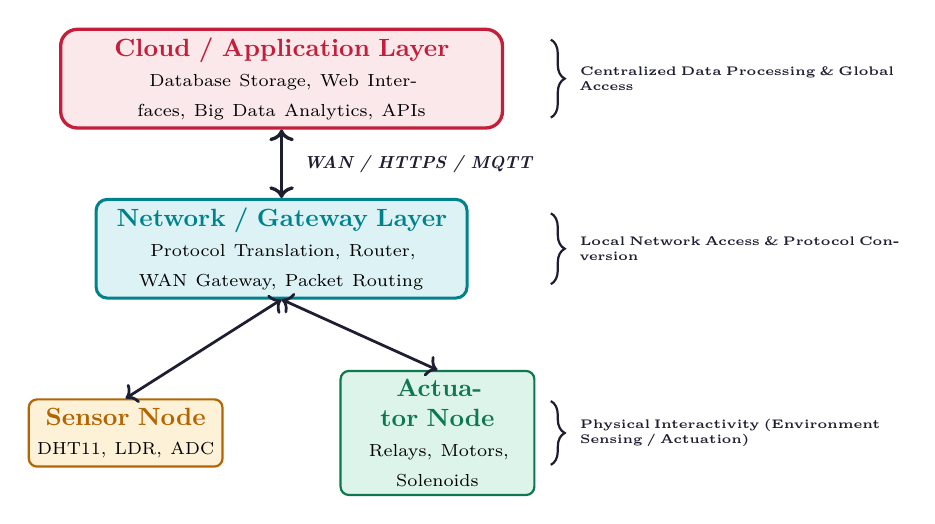
\begin{tikzpicture}[scale=0.9, transform shape]
  % Cloud Layer (Top)
  \node[draw=myred, fill=hdrred, rounded corners=6pt, line width=1.2pt, text width=6.0cm, align=center, minimum height=1.1cm] (cloud) at (0,4.8) {
    \textbf{\color{myred}Cloud / Application Layer}\\
    \scriptsize Database Storage, Web Interfaces, Big Data Analytics, APIs
  };

  % Gateway Layer (Middle)
  \node[draw=myteal, fill=hdrteal, rounded corners=4pt, line width=1.1pt, text width=5.0cm, align=center, minimum height=1.0cm] (gate) at (0,2.4) {
    \textbf{\color{myteal}Network / Gateway Layer}\\
    \scriptsize Protocol Translation, Router, WAN Gateway, Packet Routing
  };

  % Edge Nodes (Bottom)
  \node[draw=myamber, fill=hdramber, rounded corners=3pt, line width=0.8pt, text width=2.5cm, align=center, minimum height=0.9cm] (sensor) at (-2.2,-0.2) {
    \textbf{\color{myamber}Sensor Node}\\
    \scriptsize DHT11, LDR, ADC
  };

  \node[draw=mygreen, fill=hdrgreen, rounded corners=3pt, line width=0.8pt, text width=2.5cm, align=center, minimum height=0.9cm] (actuator) at (2.2,-0.2) {
    \textbf{\color{mygreen}Actuator Node}\\
    \scriptsize Relays, Motors, Solenoids
  };

  % Connections
  \draw[arrow, <->, line width=1.2pt, color=mydark] (cloud) -- node[right=5pt, font=\scriptsize\itshape\bfseries] {WAN / HTTPS / MQTT} (gate);
  \draw[arrow, <->, line width=1.0pt, color=mydark] (gate.south) -- (sensor.north);
  \draw[arrow, <->, line width=1.0pt, color=mydark] (gate.south) -- (actuator.north);

  % Labels/Side brackets - Vertically aligned at X=3.8
  \draw[thick, decoration={brace, amplitude=5pt}, decorate, color=mydark] (3.8, 5.35) -- (3.8, 4.25) 
    node[midway, right=8pt, font=\tiny\bfseries, text width=4.5cm, align=left] {Centralized Data Processing \& Global Access};

  \draw[thick, decoration={brace, amplitude=5pt}, decorate, color=mydark] (3.8, 2.90) -- (3.8, 1.90) 
    node[midway, right=8pt, font=\tiny\bfseries, text width=4.5cm, align=left] {Local Network Access \& Protocol Conversion};

  \draw[thick, decoration={brace, amplitude=5pt}, decorate, color=mydark] (3.8, 0.25) -- (3.8, -0.65) 
    node[midway, right=8pt, font=\tiny\bfseries, text width=4.5cm, align=left] {Physical Interactivity (Environment Sensing / Actuation)};
\end{tikzpicture}
\end{tcolorbox}

\subsection{Enchanted Objects}
The term \textbf{Enchanted Objects}, coined by MIT media lab researcher David Rose, refers to ordinary physical objects that are enhanced with localized, ambient technology to display information or react to user actions without demanding their full cognitive attention.
\begin{itemize}[leftmargin=*, itemsep=2pt]
  \item Instead of forcing users to look at a glowing smartphone screen, information is embedded naturally into the physical environment.
  \item \textbf{Example:} An \textit{Ambient Orb} that glows red if the stock market goes down, or blue if it goes up. The information is consumed at a glance, blending into the background.
\end{itemize}

David Rose classifies these objects according to \textbf{six fundamental human desires}:
\begin{enumerate}[leftmargin=*, itemsep=2.5pt]
  \item \textbf{Omniscience (All-Knowing):} Objects that provide information, such as the \textit{Ambient Umbrella} that glows when it is going to rain.
  \item \textbf{Telepathy (Communication):} Objects that allow remote emotional connection, like \textit{connected lamps} that light up when touched by a loved one.
  \item \textbf{Safekeeping (Protection):} Objects that track security, like smart door locks or GPS-connected wallets.
  \item \textbf{Health and Vitality:} Wearables or pill bottles that track dosage compliance and body vitals.
  \item \textbf{Teleportation (Locomotion):} Devices that bridge spatial distance, such as smart cameras or remote-controlled vehicles.
  \item \textbf{Expression (Creativity):} Instruments and smart surfaces that adapt dynamically to user expressions.
\end{enumerate}

\subsection{Who is Making the Internet of Things?}
The IoT ecosystem is built by a diverse group of creators across three main levels:
\begin{itemize}[leftmargin=*, itemsep=3.0pt]
  \item \textbf{Makers and Hobbyists:} Individuals using open-source hardware (Arduino, Raspberry Pi) and software libraries to build custom DIY projects. They drive rapid community innovation.
  \item \textbf{Startups:} Lean companies developing niche connected products (e.g. smart pet feeders, fitness wearables) and leveraging crowdfunding to prove market demand.
  \item \textbf{Tech Giants and Enterprises:} Large corporations (like Bosch, Cisco, Siemens, Google, Apple, and AWS) that design industrial IoT (IIoT) platforms, establish global protocols, and build massive cloud infrastructure to manage billions of nodes.
\end{itemize}


% ===============================================================================
\section{Design Principles for Connected Devices}
% ===============================================================================

Designing connected products requires moving away from the mouse-and-keyboard paradigm toward natural physical interfaces.

\subsection{Calm and Ambient Technology}
\begin{tcolorbox}[defbox, title={Calm Technology}]
  \textbf{Calm Technology}, formulated by Mark Weiser and John Seely Brown, is hardware/software design that informs the user but remains in the periphery of their attention, moving smoothly between the center and the margin of user focus.
\end{tcolorbox}
\begin{itemize}[leftmargin=*, itemsep=2.5pt]
  \item \textbf{Periphery Concept:} The human brain processes peripheral cues constantly (like the hum of an engine or wind blowing). Calm design uses these peripheral channels to present digital information, minimizing cognitive load.
  \item \textbf{Ambient Displays:} Use light, sound, or physical motion to convey information subtly (e.g., a smart umbrella handle that glows when rain is in the local forecast).
\end{itemize}

Mark Weiser and John Seely Brown characterized the shift in computing history across three main eras:
\begin{itemize}[leftmargin=*, itemsep=2.5pt]
  \item \textbf{Mainframe Era:} One computer shared by many people. High complexity and high cognitive distance.
  \item \textbf{Personal Computer (PC) Era:} One computer per person. Active screen attention, leading to information overload.
  \item \textbf{Ubiquitous/Calm Computing Era:} Many computers per person. Technology recedes into the physical background, operating in our peripheral attention.
\end{itemize}

\subsection{Magic as Metaphor}
When designing connected objects, users often conceptualize digital capabilities as ``magic'' (e.g. a mirror that displays weather, or a key that tracks its location).
\begin{itemize}[leftmargin=*, itemsep=2pt]
  \item Metaphors from fairy tales (such as crystal balls, magic wands, and mirrors) serve as design patterns for natural user interfaces.
  \item The technology should remain invisible; the user interacts directly with the physical object, not the screen/interface.
\end{itemize}

\subsection{Web Thinking for Connected Devices}
Applying Web principles to physical hardware is called the \textbf{Web of Things (WoT)}:
\begin{itemize}[leftmargin=*, itemsep=3pt]
  \item \textbf{Loose Coupling:} Connected devices should be modular and independent. Changing the cloud backend should not brick the physical device.
  \item \textbf{RESTful Architectures:} Representing physical actions as resources using standard HTTP verbs (e.g., `POST /livingroom/light` to turn on a lamp).
  \item \textbf{Open Standards:} Prefer open APIs, JSON, and TCP/IP protocols over proprietary closed stacks to prevent vendor lock-in.
\end{itemize}

\subsection{Affordances}
\begin{tcolorbox}[defbox, title={Affordance}]
  An \textbf{Affordance} is the physical property of an object that suggests how it should be used or interacted with (e.g., a handle affords pulling, and a button affords pushing).
\end{tcolorbox}
In IoT design, physical affordances must match digital functions. If a smart lamp requires twisting to dim, the physical knob must feel like a dimming control, and the digital latency must be low enough to maintain the illusion of physical causality.

\newpage

% ═══════════════════════════════════════════════════════════════════════════════
% QUICK REVISION PAGE
% ═══════════════════════════════════════════════════════════════════════════════
\begin{center}
  {\large\bfseries\color{myred} Quick Revision — Module 1}\\[3pt]
  {\small\color{mydark} Introduction \& Design Principles $|$ OE-EC803A}
\end{center}
\noindent{\color{myred}\rule{\linewidth}{1.2pt}}
\vspace{8pt}

\begin{tcolorbox}[defbox, title={\textbf{One-Line Definitions}}]
\begin{itemize}[leftmargin=*, itemsep=3pt, topsep=0pt]
  \item \textbf{IoT:} Interconnected network of physical objects embedded with sensors and connectivity.
  \item \textbf{Enchanted Object:} A physical item enhanced with subtle digital properties to make it feel ``magical.''
  \item \textbf{Calm Technology:} Technology designed to sit in the user's peripheral attention until needed.
  \item \textbf{Affordance:} Physical shape or properties of an object suggesting its interface usage.
  \item \textbf{Web of Things (WoT):} Extending Web standards (HTTP, REST, JSON) to integrate IoT devices.
\end{itemize}
\end{tcolorbox}

\vspace{6pt}

\begin{tcolorbox}[exambox, title={\textbf{Frequently Asked / Viva Questions}}]
\begin{enumerate}[leftmargin=*, topsep=0pt, label=\textbf{Q\arabic*.}, itemsep=6pt]
  \item \Q{What is the difference between IoT and M2M?}
        M2M (Machine-to-Machine) is usually point-to-point, closed-network hardware communication over dedicated links (e.g., cellular/radio), while IoT is a globally open network of heterogeneous devices interacting using standardized IP protocols.
        
  \item \Q{Explain David Rose's concept of ``Enchanted Objects.''}
        David Rose describes enchanted objects as ordinary physical items (like mirrors, umbrellas, or pens) embedded with simple, glanceable digital capabilities. Instead of screens commanding our focus, these items use ambient cues to blend information into our physical surroundings.
        
  \item \Q{How does Calm Technology process information?}
        Calm technology relies on the human brain's ability to process peripheral cues. It displays digital status parameters in the margins of attention (like an ambient light color change). If the parameter changes critically, it draws the user's focus to the center.
        
  \item \Q{What is an ``affordance'' in physical device design?}
        An affordance is a visual or physical cue indicating how an object operates. For example, a round dial suggests rotation. In IoT design, physical controls must afford their digital actions to make the interface intuitive.
        
  \item \Q{What does the phrase ``Magic as Metaphor'' mean in IoT design?}
        It means designing connected objects that behave like mythical items (e.g., a compass pointing to a friend, or a key that remembers where it is). It simplifies the user's mental model by mapping complex technology to familiar magical concepts.
        
  \item \Q{Why is open API standard design critical in IoT?}
        Proprietary closed APIs isolate devices and lead to vendor lock-in. If the vendor shuts down their cloud server, the device is bricked. Open APIs and standards allow interoperability and support local control independent of specific cloud stacks.
        
  \item \Q{What is the Web of Things (WoT)?}
        The Web of Things is a framework that uses standard web application layer protocols (HTTP, REST, WebSockets, JSON) to interface and control IoT edge hardware, making them as easy to access as regular web documents.
        
  \item \Q{What are the typical layers of an IoT system?}
        (1) Perception/Edge Layer (collects data via sensors), (2) Network/Gateway Layer (handles routing and protocol translation), and (3) Application/Cloud Layer (analyzes data and executes business logic).
\end{enumerate}
\end{tcolorbox}

\vspace{6pt}

\begin{tcolorbox}[tikzbox, title={\textbf{Comparison Snapshot}}]
\textbf{Calm Technology vs. Screen-Based Technology:}\par\vspace{6pt}\noindent
{\renewcommand{\arraystretch}{1.35}%
\begin{tabularx}{\linewidth}{|B{3.2cm}|Y|Y|}
\hline
\textbf{Feature} & \textbf{Calm Technology} & \textbf{Screen-Based Technology} \\
\hline
Attention Demand & Relies on peripheral attention. & Demands full visual and cognitive attention. \\
\hline
Context Integration & Integrates seamlessly into physical objects. & Requires dedicated, isolated visual displays. \\
\hline
Cognitive Load & Low; processes cues ambiently. & High; causes screen fatigue and information overload. \\
\hline
Example & Smart umbrella glowing when rain is near. & Phone notification showing rain forecast percentage. \\
\hline
\end{tabularx}}
\end{tcolorbox}


% -- Module 2 -----------------------------------------------------------------
\modulestart{2}{Internet Communications Overview}

\section{Internet Communications Overview}
% ===============================================================================

IoT devices rely on internet communication stacks to transmit sensor data and receive commands. The dominant model is the \textbf{TCP/IP Protocol Suite}.

\begin{tcolorbox}[defbox, title={TCP/IP Protocol Suite}]
  The \textbf{TCP/IP Protocol Suite} is a four-layer conceptual model for network communication. It consists of the Link Layer, Internet Layer (IP), Transport Layer (TCP/UDP), and Application Layer (HTTP/CoAP/MQTT).
\end{tcolorbox}

\subsection{Transport Layer: TCP vs. UDP}
IoT edge devices choose transport protocols based on power, latency, and reliability requirements:
\begin{itemize}[leftmargin=*, itemsep=3pt]
  \item \textbf{TCP (Transmission Control Protocol):} A connection-oriented, reliable protocol. It guarantees in-order delivery of data using handshakes, acknowledgments, and retransmission mechanisms. The drawback is high header overhead (20 bytes) and higher power consumption, which is challenging for constrained devices.
  \item \textbf{UDP (User Datagram Protocol):} A connectionless, lightweight transport protocol. It sends packets (datagrams) without verifying if the receiver is ready or if the packets arrive. It has minimal header overhead (8 bytes) and low latency, making it ideal for battery-powered sensor nodes (often combined with CoAP).
\end{itemize}

\begin{tcolorbox}[examplebox, title={TCP Three-Way Handshake Connection Lifecycle}]
  Establishing a reliable TCP connection requires a three-way handshake before any application data is sent:
  \begin{enumerate}[leftmargin=*, itemsep=2pt]
    \item \textbf{SYN (Synchronize):} The client sends a segment with the SYN flag set and an initial sequence number ($Seq = x$) to request a connection.
    \item \textbf{SYN-ACK (Synchronize-Acknowledge):} The server replies with a segment where both SYN and ACK flags are set, acknowledging the client's sequence ($Ack = x+1$) and sending its own sequence number ($Seq = y$).
    \item \textbf{ACK (Acknowledge):} The client sends a final segment acknowledging the server's sequence ($Ack = y+1$). The connection is now \texttt{ESTABLISHED}.
  \end{enumerate}
  For teardown, a four-step handshake using \textbf{FIN} (Finish) and \textbf{ACK} segments is executed to close both directions of the full-duplex link.
\end{tcolorbox}

% ===============================================================================
\section{IP Addressing and Routing}
% ===============================================================================

Every node connected to the Internet needs a unique address for routing packets.

\subsection{IP Addresses and DNS}
\begin{itemize}[leftmargin=*, itemsep=3pt]
  \item \textbf{DNS (Domain Name System):} Translates human-readable domain names (e.g. `api.weather.com`) into machine-readable IP addresses.
  \item \textbf{Static IP Assignment:} The address is manually configured on the device. Ideal for servers and local gateways but hard to scale.
  \item \textbf{Dynamic IP Assignment (DHCP):} A DHCP server automatically assigns a temporary IP address to devices when they connect to the network. Essential for scaling large fleets of consumer IoT devices.
\end{itemize}

\subsection{IPv4 vs. IPv6 in IoT}
\begin{tcolorbox}[defbox, title={IPv6 Importance in IoT}]
  \textbf{IPv6 (Internet Protocol version 6)} uses $128$-bit addresses, yielding $3.4 \times 10^{38}$ unique addresses, compared to the $32$-bit ($4.3$ billion) address pool of \textbf{IPv4}. IPv6 is critical for IoT because it allows every smart object on Earth to have a unique, globally routable public IP address, eliminating the need for complex Network Address Translation (NAT) gateways.
\end{tcolorbox}

\par\vspace{6pt}\noindent
{\renewcommand{\arraystretch}{1.3}%
\begin{tabularx}{\linewidth}{|B{3.0cm}|Y|Y|}
\hline
\textbf{Feature} & \textbf{IPv4 Header} & \textbf{IPv6 Header} \\
\hline
Header Size & Variable ($20$ to $60$ bytes). & Fixed ($40$ bytes). \\
\hline
Address Size & $32$ bits ($4$ bytes). & $128$ bits ($16$ bytes). \\
\hline
Fields Count & $12$ fields. & Only $8$ fields. \\
\hline
Checksum Field & Present (must be recomputed at each hop). & Removed (handled by Layer 2 and Layer 4). \\
\hline
Fragmentation & Handled by routers and sending hosts. & Handled only by sending hosts (PMTU discovery). \\
\hline
\end{tabularx}}

\subsection{MAC Addresses}
A \textbf{MAC (Media Access Control) Address} is a unique, 48-bit physical hardware identifier burned into a network interface card (NIC) by the manufacturer. While IP addresses change based on location/network, the MAC address remains constant, uniquely identifying the hardware locally.

\subsection{Ports}
\textbf{Ports} are 16-bit logical identifiers at the Transport Layer used to route data packets to specific software applications running on a host. Common IoT port assignments include HTTP (80), MQTT (1883), CoAP (5683), and HTTPS/MQTTS (443/8883).

% ===============================================================================
\section{Application Layer Protocols in IoT}
% ===============================================================================

To handle resource constraints (memory, bandwidth, power), specialized application layer protocols are used instead of heavy web HTTP.

\subsection{MQTT (Message Queuing Telemetry Transport)}
MQTT is a lightweight, broker-based publish-subscribe messaging protocol designed for high-latency, low-bandwidth networks.
\begin{itemize}[leftmargin=*, itemsep=2.5pt]
  \item \textbf{Clients:} Publish messages to topics or subscribe to topics to receive messages.
  \item \textbf{Broker:} The central server that receives published messages and distributes them to all subscribed clients.
  \item \textbf{QoS (Quality of Service) Levels:}
        \begin{itemize}[leftmargin=*, label=$\bullet$, itemsep=3.0pt]
          \item \textit{QoS 0 (At most once):} Fire-and-forget; no handshake, no guaranteed delivery. Minimal overhead.
          \item \textit{QoS 1 (At least once):} Guaranteed delivery but duplicates may arrive.
                \begin{itemize}[leftmargin=*, label=$\circ$, itemsep=1.0pt]
                  \item Client sends a \texttt{PUBLISH} message containing a unique Packet Identifier.
                  \item Broker stores and forwards the message, replying with a \texttt{PUBACK} acknowledgment. If the client doesn't receive \texttt{PUBACK} before a timeout, it re-transmits.
                \end{itemize}
          \item \textit{QoS 2 (Exactly once):} Four-step handshake guarantees delivery with zero duplicates.
                \begin{itemize}[leftmargin=*, label=$\circ$, itemsep=1.0pt]
                  \item Client sends \texttt{PUBLISH}.
                  \item Broker stores packet ID and sends \texttt{PUBREC} (Publish Received).
                  \item Client receives \texttt{PUBREC} and sends \texttt{PUBREL} (Publish Release) to unlock broker storage.
                  \item Broker processes/distributes message, replying with \texttt{PUBCOMP} (Publish Complete).
                \end{itemize}
        \end{itemize}
\end{itemize}

\begin{tcolorbox}[tikzbox, title={MQTT Publish-Subscribe Architecture}]
\centering
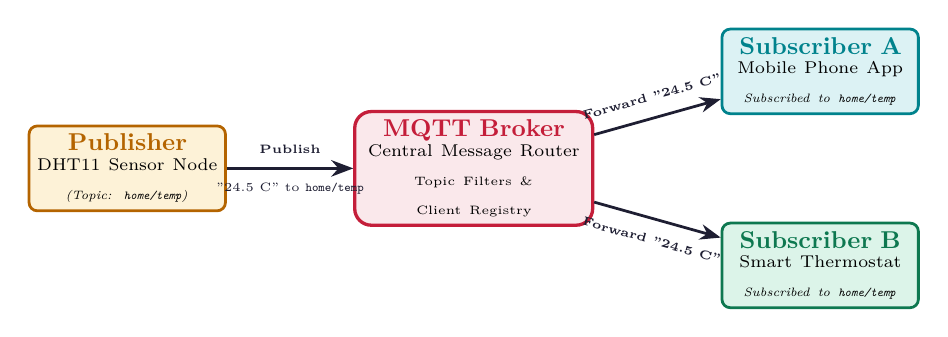
\begin{tikzpicture}[scale=0.88, transform shape]
  % Publisher (Left)
  \node[draw=myamber, fill=hdramber, rounded corners=3pt, line width=1pt, text width=2.6cm, align=center, minimum height=1.1cm] (pub) at (-5.0, 0) {
    \textbf{\color{myamber}Publisher}\\
    \scriptsize DHT11 Sensor Node\\
    \itshape\tiny (Topic: \texttt{home/temp})
  };

  % Broker (Center)
  \node[draw=myred, fill=hdrred, rounded corners=6pt, line width=1.2pt, text width=3.2cm, align=center, minimum height=1.3cm] (broker) at (0, 0) {
    \textbf{\color{myred}MQTT Broker}\\
    \scriptsize Central Message Router\\
    \tiny Topic Filters \& Client Registry
  };

  % Subscriber 1 (Top Right)
  \node[draw=myteal, fill=hdrteal, rounded corners=3pt, line width=1pt, text width=2.6cm, align=center, minimum height=1.1cm] (sub1) at (5.0, 1.4) {
    \textbf{\color{myteal}Subscriber A}\\
    \scriptsize Mobile Phone App\\
    \itshape\tiny Subscribed to \texttt{home/temp}
  };

  % Subscriber 2 (Bottom Right)
  \node[draw=mygreen, fill=hdrgreen, rounded corners=3pt, line width=1pt, text width=2.6cm, align=center, minimum height=1.1cm] (sub2) at (5.0, -1.4) {
    \textbf{\color{mygreen}Subscriber B}\\
    \scriptsize Smart Thermostat\\
    \itshape\tiny Subscribed to \texttt{home/temp}
  };

  % Connections - Straight and Sloped to avoid overlap
  \draw[arrow, line width=1.1pt] (pub) -- node[above=2pt, font=\tiny\bfseries] {Publish} node[below=2pt, font=\tiny] {"24.5 C" to \texttt{home/temp}} (broker);
  
  \draw[arrow, line width=1.0pt] (broker) -- node[midway, above=3pt, font=\tiny\bfseries, sloped] {Forward "24.5 C"} (sub1);
  \draw[arrow, line width=1.0pt] (broker) -- node[midway, below=3pt, font=\tiny\bfseries, sloped] {Forward "24.5 C"} (sub2);
\end{tikzpicture}
\end{tcolorbox}

\subsection{CoAP (Constrained Application Protocol)}
CoAP is a web transfer protocol designed for constrained nodes and networks:
\begin{itemize}[leftmargin=*, itemsep=2pt]
  \item It uses a RESTful request-response model mapping to standard HTTP methods (GET, POST, PUT, DELETE).
  \item Unlike HTTP, CoAP runs over \textbf{UDP} instead of TCP, dramatically reducing connection handshakes and packet overhead.
\end{itemize}

\begin{tcolorbox}[tikzbox, title={CoAP Request-Response over UDP}]
\centering
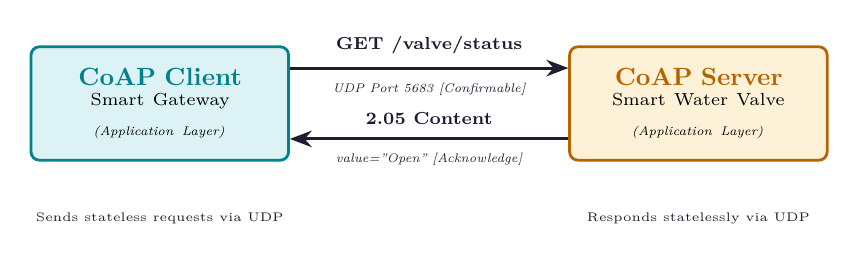
\begin{tikzpicture}[scale=0.9, transform shape]
  % Client Box
  \node[draw=myteal, fill=hdrteal, rounded corners=3pt, line width=1pt, text width=3.4cm, align=center, minimum height=1.6cm] (client) at (-3.8, 0) {
    \textbf{\color{myteal}CoAP Client}\\
    \scriptsize Smart Gateway\\
    \itshape\tiny (Application Layer)
  };

  % Server Box
  \node[draw=myamber, fill=hdramber, rounded corners=3pt, line width=1pt, text width=3.4cm, align=center, minimum height=1.6cm] (server) at (3.8, 0) {
    \textbf{\color{myamber}CoAP Server}\\
    \scriptsize Smart Water Valve\\
    \itshape\tiny (Application Layer)
  };

  % Communication flow lines - Increased gap to Y=+0.5 and Y=-0.5
  \draw[arrow, line width=1.1pt, color=mydark] ($(client.east)+(0,0.5)$) -- node[midway, above=2pt, font=\scriptsize\bfseries] {GET /valve/status} node[midway, below=2pt, font=\tiny\itshape, color=mydark] {UDP Port 5683 [Confirmable]} ($(server.west)+(0,0.5)$);
  
  \draw[arrow, line width=1.1pt, color=mydark] ($(server.west)+(0,-0.5)$) -- node[midway, above=2pt, font=\scriptsize\bfseries] {2.05 Content} node[midway, below=2pt, font=\tiny\itshape, color=mydark] {value="Open" [Acknowledge]} ($(client.east)+(0,-0.5)$);

  % Transport Layer Labels (Bottom)
  \node[below=0.6cm of client, font=\tiny, color=mydark] {Sends stateless requests via UDP};
  \node[below=0.6cm of server, font=\tiny, color=mydark] {Responds statelessly via UDP};
\end{tikzpicture}
\end{tcolorbox}

\newpage

% ═══════════════════════════════════════════════════════════════════════════════
% QUICK REVISION PAGE
% ═══════════════════════════════════════════════════════════════════════════════
\begin{center}
  {\large\bfseries\color{myred} Quick Revision — Module 2}\\[3pt]
  {\small\color{mydark} Networking \& Protocols $|$ OE-EC803A}
\end{center}
\noindent{\color{myred}\rule{\linewidth}{1.2pt}}
\vspace{8pt}

\begin{tcolorbox}[formulabox, title={\textbf{Key Protocols and Specs at a Glance}}]
\renewcommand{\arraystretch}{1.35}
\begin{tabularx}{\linewidth}{B{5.0cm} X}
  IPv4 Address Length & $32$ bits ($4$ bytes) $\rightarrow$ e.g., $192.168.1.10$ \\[4pt]
  IPv6 Address Length & $128$ bits ($16$ bytes) $\rightarrow$ e.g., $2001:0db8:85a3::8a2e:0370:7334$ \\[4pt]
  MQTT Ports & Port $1883$ (TCP, unencrypted) and Port $8883$ (Encrypted SSL/TLS) \\[4pt]
  CoAP Port & Port $5683$ (UDP, unencrypted) and Port $5684$ (DTLS security)
\end{tabularx}
\end{tcolorbox}

\vspace{6pt}

\begin{tcolorbox}[defbox, title={\textbf{One-Line Definitions}}]
\begin{itemize}[leftmargin=*, itemsep=3pt, topsep=0pt]
  \item \textbf{TCP/IP Model:} A standardized suite of communication protocols used to connect devices on the internet.
  \item \textbf{QoS (MQTT):} Quality of Service agreement determining the reliability and handshake level of message delivery.
  \item \textbf{MAC Address:} A permanent, unique physical address burned into the hardware interface card.
  \item \textbf{CoAP:} A lightweight RESTful transfer protocol running over UDP for constrained networks.
  \item \textbf{DHCP:} An automated protocol that dynamically assigns IP configurations to joining devices.
\end{itemize}
\end{tcolorbox}

\vspace{6pt}

\begin{tcolorbox}[exambox, title={\textbf{Frequently Asked / Viva Questions}}]
\begin{enumerate}[leftmargin=*, topsep=0pt, label=\textbf{Q\arabic*.}, itemsep=6pt]
  \item \Q{Why is TCP preferred for applications like web browsing, but UDP is preferred for real-time sensor streams?}
        TCP is connection-oriented and guarantees that every packet is received in order through acknowledgments. This prevents page layout distortion but adds latency. UDP sends packets without handshakes. It is faster, has less overhead, and is ideal for sensor streams where losing an occasional packet is acceptable but latency must be low.
        
  \item \Q{Why is IPv6 essential for the growth of IoT?}
        IPv4 only supports $4.3$ billion addresses, which have already been exhausted. IoT connects tens of billions of smart objects. IPv6 provides $128$-bit addresses ($3.4 \times 10^{38}$), allowing every individual device to have a globally unique IP address without routing behind NAT gateways.
        
  \item \Q{How does the publish-subscribe model in MQTT differ from the client-server model in HTTP?}
        In HTTP (client-server), clients pull data by initiating requests, requiring both devices to be online and active at the same time (tight temporal coupling). In MQTT (publish-subscribe), clients publish data to a broker, which pushes it to subscribers. The publisher and subscriber do not know each other and are decoupled.
        
  \item \Q{Explain the three QoS levels in MQTT.}
        (1) QoS 0 (At most once): Sends the message once with zero handshakes. Best for high-frequency, non-critical data. (2) QoS 1 (At least once): Delivers the message but might send duplicates. Requires a puback packet. (3) QoS 2 (Exactly once): Guarantees the message is received exactly once using a 4-packet exchange.
        
  \item \Q{What is CoAP, and what transport layer protocol does it use?}
        CoAP (Constrained Application Protocol) is a lightweight web transfer protocol designed for resource-constrained IoT nodes. It mirrors the RESTful model of HTTP (GET/POST) but runs over UDP, reducing header overhead and handshake latency.
        
  \item \Q{Why do we need a DNS server?}
        Humans read names (like `io.adafruit.com`), but routing hardware only reads binary IP addresses. The DNS server acts as a directory that looks up the domain name and returns the active IP address.
        
  \item \Q{Explain the difference between static and dynamic IP assignment.}
        Static IP addresses are configured manually and remain fixed, which is useful for local gateways. Dynamic IP addresses are leased temporarily from a pool by a DHCP server, which simplifies administration for large scale deployments.
        
  \item \Q{What is the difference between a MAC address and an IP address?}
        A MAC address is a physical, 48-bit identifier assigned permanently to the device hardware by the manufacturer. An IP address is a logical address assigned dynamically by the network to route packets across subnets.
\end{enumerate}
\end{tcolorbox}

\vspace{6pt}

\begin{tcolorbox}[tikzbox, title={\textbf{Comparison Snapshot}}]
\textbf{MQTT vs. CoAP vs. HTTP:}\par\vspace{6pt}\noindent
{\renewcommand{\arraystretch}{1.35}%
\begin{tabularx}{\linewidth}{|B{3.2cm}|Y|Y|Y|}
\hline
\textbf{Feature} & \textbf{MQTT} & \textbf{CoAP} & \textbf{HTTP} \\
\hline
Architecture & Publish / Subscribe & Request / Response (REST) & Request / Response (REST) \\
\hline
Transport Layer & TCP & UDP & TCP \\
\hline
Header Size & Minimal (2 bytes) & Small (4 bytes) & Large (Hundreds of bytes) \\
\hline
Security & SSL / TLS & DTLS & SSL / TLS (HTTPS) \\
\hline
Use Case & Continuous telemetry streams. & Low-power, event-driven queries. & Heavy dashboard interfaces. \\
\hline
\end{tabularx}}
\end{tcolorbox}


% -- Module 3 -----------------------------------------------------------------
\modulestart{3}{Thinking About Prototyping}

\section{Thinking About Prototyping}
% ===============================================================================

Prototyping is the iterative process of quickly assembling a working model of a device to test assumptions and functionality before entering mass manufacturing.

\subsection{Prototyping Considerations}
\begin{itemize}[leftmargin=*, itemsep=3pt]
  \item \textbf{Sketching:} Fast, non-functional drawings to visualize hardware forms and user flows.
  \item \textbf{Familiarity:} Choosing tools the designer already knows (e.g. Arduino IDE) to reduce development time, even if other tools are mathematically more optimal.
  \item \textbf{Costs vs. Ease:} Fast prototyping tools (like jumper wires and breadboards) are cheap and easy, but produce bulky, fragile systems. Production-ready designs require custom PCBs.
  \item \textbf{Open Source vs. Closed Source:} Open hardware/software allows developers to adapt existing code libraries and hardware schematics, tapping into massive global communities.
\end{itemize}

% ===============================================================================
\section{Basic Electronics for IoT}
% ===============================================================================

IoT edge nodes interface directly with the physical world using sensors and actuators.

\subsection{Basic Quantities}
\begin{tcolorbox}[formulabox, title={Ohm's Law and Electrical Power}]
  \textbf{Ohm's Law} relates voltage ($V$), current ($I$), and resistance ($R$):
  \begin{equation}
    V = I \cdot R
  \end{equation}
  Electrical power ($P$) in watts is given by:
  \begin{equation}
    P = V \cdot I = I^2 \cdot R
  \end{equation}
\end{tcolorbox}

\begin{tcolorbox}[formulabox, title={Voltage Dividers and Analog-to-Digital Conversion (ADC)}]
  \textbf{Voltage Divider Formula:} Reduces a high analog voltage ($V_{\text{in}}$) to a safe range ($V_{\text{out}}$) for microcontroller pins:
  \begin{equation}
    V_{\text{out}} = V_{\text{in}} \cdot \left( \frac{R_2}{R_1 + R_2} \right)
  \end{equation}
  \textbf{ADC Resolution:} Quantizes an analog voltage into a digital integer. For an $n$-bit ADC with reference voltage $V_{\text{ref}}$, the step size (Resolution) is:
  \begin{equation}
    \text{Step Size (LSB)} = \frac{V_{\text{ref}}}{2^n}
  \end{equation}
  The measured digital value $D$ for an input voltage $V_{\text{in}}$ is:
  \begin{equation}
    D = \text{round}\left( \frac{V_{\text{in}}}{\text{Step Size}} \right) = \text{round}\left( V_{\text{in}} \cdot \frac{2^n}{V_{\text{ref}}} \right)
  \end{equation}
\end{tcolorbox}

\subsection{Signals and Interface Elements}
\begin{itemize}[leftmargin=*, itemsep=3.5pt]
  \item \textbf{Digital vs. Analog:} Digital signals are binary ($0$ or $1$, representing $0\text{V}$ and $3.3\text{V}/5\text{V}$). Analog signals vary continuously (e.g., LDR resistance changing with light).
  \item \textbf{PWM (Pulse Width Modulation):} Mimics analog outputs from a digital pin by switching the pin ON and OFF very rapidly. The ratio of ON time to the period is called the \textbf{Duty Cycle ($D$)}:
        \begin{equation}
          V_{\text{eff}} = D \cdot V_{\text{max}}
        \end{equation}
  \item \textbf{DHT11 Sensor:} A digital sensor measuring temperature and humidity, sending data over a single-wire digital protocol.
  \item \textbf{Relay:} An electromagnetic switch allowing a low-power microcontroller pin to switch high-voltage/high-current AC devices.
\end{itemize}

% ===============================================================================
\section{Prototyping Embedded Platforms}
% ===============================================================================

IoT designs select hardware platforms based on processing power, OS requirements, and connectivity.

\subsection{Embedded Computing Basics}
\begin{itemize}[leftmargin=*, itemsep=3pt]
  \item \textbf{Microcontroller (MCU):} A single integrated circuit containing a CPU, RAM, Flash memory, and I/O peripherals (GPIO, ADC, SPI, I2C). Low-power, real-time execution. Example: ATmega328P.
  \item \textbf{Microprocessor (MPU):} Contains only the CPU. Requires external RAM, Flash, and support ICs. Runs complex Operating Systems (Linux). High power consumption. Example: ARM Cortex-A72.
\end{itemize}

\begin{tcolorbox}[tikzbox, title={Microcontroller Internal Architecture (System Bus Model)}]
\centering
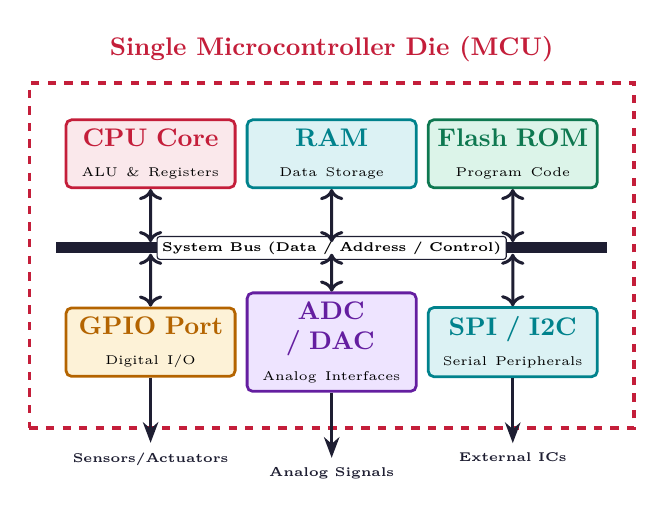
\begin{tikzpicture}[scale=0.92, transform shape]
  % System Bus (Central Backbone) - Label placed in center with white background to avoid boundary collision
  \draw[line width=4pt, color=mydark] (-3.8, 0) -- (3.8, 0);
  \node[font=\tiny\bfseries, fill=white, draw=mydark, rounded corners=1pt, inner sep=2pt] at (0,0) {System Bus (Data / Address / Control)};

  % Blocks above bus
  \node[draw=myred, fill=hdrred, rounded corners=2pt, line width=1pt, text width=2.1cm, align=center, minimum height=0.9cm] (cpu) at (-2.5, 1.3) {
    \textbf{\color{myred}CPU Core}\\
    \tiny ALU \& Registers
  };
  
  \node[draw=myteal, fill=hdrteal, rounded corners=2pt, line width=1pt, text width=2.1cm, align=center, minimum height=0.9cm] (ram) at (0, 1.3) {
    \textbf{\color{myteal}RAM}\\
    \tiny Data Storage
  };

  \node[draw=mygreen, fill=hdrgreen, rounded corners=2pt, line width=1pt, text width=2.1cm, align=center, minimum height=0.9cm] (flash) at (2.5, 1.3) {
    \textbf{\color{mygreen}Flash ROM}\\
    \tiny Program Code
  };

  % Blocks below bus
  \node[draw=myamber, fill=hdramber, rounded corners=2pt, line width=1pt, text width=2.1cm, align=center, minimum height=0.9cm] (gpio) at (-2.5, -1.3) {
    \textbf{\color{myamber}GPIO Port}\\
    \tiny Digital I/O
  };

  \node[draw=mypurple, fill=hdrpurple, rounded corners=2pt, line width=1pt, text width=2.1cm, align=center, minimum height=0.9cm] (adc) at (0, -1.3) {
    \textbf{\color{mypurple}ADC / DAC}\\
    \tiny Analog Interfaces
  };

  \node[draw=myteal, fill=hdrteal, rounded corners=2pt, line width=1pt, text width=2.1cm, align=center, minimum height=0.9cm] (serial) at (2.5, -1.3) {
    \textbf{\color{myteal}SPI / I2C}\\
    \tiny Serial Peripherals
  };

  % Bus taps (arrows)
  \draw[arrow, <->, line width=1.1pt] (cpu) -- (cpu |- 0, 0.08);
  \draw[arrow, <->, line width=1.1pt] (ram) -- (ram |- 0, 0.08);
  \draw[arrow, <->, line width=1.1pt] (flash) -- (flash |- 0, 0.08);
  \draw[arrow, <->, line width=1.1pt] (gpio) -- (gpio |- 0, -0.08);
  \draw[arrow, <->, line width=1.1pt] (adc) -- (adc |- 0, -0.08);
  \draw[arrow, <->, line width=1.1pt] (serial) -- (serial |- 0, -0.08);

  % Boundary Box (MCU Die)
  \node[draw=myred, dashed, line width=1.2pt, fit=(cpu) (ram) (flash) (gpio) (adc) (serial), inner sep=0.45cm] (mcu) {};
  \node[above=0.15cm of mcu, font=\bfseries\color{myred}] {Single Microcontroller Die (MCU)};
  
  % External interfaces - Lengthened arrows to Y=-2.8 to clear dashed boundary
  \draw[arrow, line width=1pt] (gpio.south) -- ++(0, -0.9) node[below, font=\tiny\bfseries] {Sensors/Actuators};
  \draw[arrow, line width=1pt] (adc.south) -- ++(0, -0.9) node[below, font=\tiny\bfseries] {Analog Signals};
  \draw[arrow, line width=1pt] (serial.south) -- ++(0, -0.9) node[below, font=\tiny\bfseries] {External ICs};
\end{tikzpicture}
\end{tcolorbox}

\subsection{Hardware Platforms Overview}
\begin{enumerate}[leftmargin=*, itemsep=4.0pt]
  \item \textbf{Arduino (Microcontroller-Based):} 
        \begin{itemize}[leftmargin=*, label=$\bullet$, itemsep=1.5pt]
          \item Powered by the \textbf{ATmega328P} 8-bit MCU operating at $16\text{ MHz}$, containing $32\text{ KB}$ Flash, $2\text{ KB}$ SRAM, and $1\text{ KB}$ EEPROM.
          \item Programmed in C++ using bare-metal register manipulation (e.g. setting \texttt{DDRB |= (1 << 5)} to configure Pin 13 as output, and writing to \texttt{PORTB} to toggle pins) compiled via \texttt{avr-gcc}.
          \item Ideal for low-power sleep modes ($<15\ \mu\text{A}$ in power-down mode) and deterministic, timing-critical sensor polling.
        \end{itemize}
  \item \textbf{Raspberry Pi (Single-Board Computer):}
        \begin{itemize}[leftmargin=*, label=$\bullet$, itemsep=1.5pt]
          \item Powered by a Broadcom \textbf{System-on-Chip (SoC)} containing a quad-core 64-bit ARM Cortex processor, up to $8\text{ GB}$ RAM, and GPU.
          \item Runs a fully pre-emptive Linux OS (Raspberry Pi OS) from an SD card. This introduces OS scheduling latency (non-deterministic) but allows full network stacks, file systems, and high-level runtimes (Python, Node.js).
          \item Used as local edge gateways, database hosts, and for CPU-intensive tasks like computer vision or edge AI inference.
        \end{itemize}
  \item \textbf{BeagleBone Black (PRU Co-processors):}
        \begin{itemize}[leftmargin=*, label=$\bullet$, itemsep=1.5pt]
          \item Features a $1\text{ GHz}$ ARM Cortex-A8 processor running Linux, augmented with two auxiliary \textbf{PRUs (Programmable Real-Time Units)}.
          \item Each PRU is a 32-bit RISC core operating at $200\text{ MHz}$ with direct access to hardware I/O pins and shared RAM, operating independently of the Linux kernel's interrupts or process schedules.
          \item Solves the "non-deterministic OS" issue, enabling sub-microsecond GPIO toggling, precise high-speed industrial motor control, and custom hardware protocol decoding.
        \end{itemize}
  \item \textbf{Electric Imp (Cloud-Integrated Module):}
        \begin{itemize}[leftmargin=*, label=$\bullet$, itemsep=1.5pt]
          \item A secure hardware module featuring an ARM Cortex processor and Wi-Fi interface.
          \item Utilizes a \textbf{Cloud-Device Split Model}: Code is split into a local \textit{Device} script (interfacing with pins) and a cloud-based \textit{Agent} script (running in Electric Imp's secure VM, handling HTTPS/OAuth).
          \item Programmed in the \textbf{Squirrel} scripting language. Features built-in secure boot, automated secure OTA firmware updates, and managed cloud routing.
        \end{itemize}
  \item \textbf{Mobile Phone and Tablets (Sensors \& Application Runtimes):}
        \begin{itemize}[leftmargin=*, label=$\bullet$, itemsep=1.5pt]
          \item High-performance mobile devices equipped with gigabytes of RAM, multi-core CPUs, and multi-Gbps cellular/Wi-Fi/Bluetooth networking.
          \item Host rich integrated sensors (dual-frequency GPS, 3-axis accelerometers, gyroscopes, magnetometers, ambient light sensors, cameras, and microphones).
          \item Used for rapid application-level prototyping, mobile dashboard display, and utilizing internal sensors as edge input devices.
        \end{itemize}
  \item \textbf{Plug Computing (Always-On Mini-Servers):}
        \begin{itemize}[leftmargin=*, label=$\bullet$, itemsep=1.5pt]
          \item Compact, wall-plug-sized, always-on servers containing a low-power MPU (e.g. Marvell Kirkwood ARM), RAM, flash storage, and an Ethernet/Wi-Fi connection.
          \item Run headless Linux server distributions (e.g., Debian).
          \item Act as quiet, unobtrusive, low-power local gateways, print servers, and local home automation hub controllers.
        \end{itemize}
\end{enumerate}

\newpage

% ═══════════════════════════════════════════════════════════════════════════════
% QUICK REVISION PAGE
% ═══════════════════════════════════════════════════════════════════════════════
\begin{center}
  {\large\bfseries\color{myred} Quick Revision — Module 3}\\[3pt]
  {\small\color{mydark} Embedded Hardware Platforms $|$ OE-EC803A}
\end{center}
\noindent{\color{myred}\rule{\linewidth}{1.2pt}}
\vspace{8pt}

\begin{tcolorbox}[formulabox, title={\textbf{Key Formulas and Metrics at a Glance}}]
\renewcommand{\arraystretch}{1.35}
\begin{tabularx}{\linewidth}{B{5.0cm} X}
  Ohm's Law & $V = I \cdot R \quad (\text{Volts, Amperes, Ohms})$ \\[4pt]
  Power dissipation & $P = V \cdot I = I^2 \cdot R \quad (\text{Watts})$ \\[4pt]
  PWM Effective Voltage & $V_{\text{eff}} = D \cdot V_{\text{max}} \quad (D = \text{Duty Cycle } \in [0, 1])$ \\[4pt]
  ADC Resolution & $V_{\text{step}} = \dfrac{V_{\text{ref}}}{2^N - 1} \quad (N\text{-bit Analog-to-Digital Converter})$
\end{tabularx}
\end{tcolorbox}

\vspace{6pt}

\begin{tcolorbox}[defbox, title={\textbf{One-Line Definitions}}]
\begin{itemize}[leftmargin=*, itemsep=3pt, topsep=0pt]
  \item \textbf{Microcontroller:} An IC integrating CPU, memory, and peripheral interfaces on a single chip.
  \item \textbf{Single-Board Computer:} A complete computer built on a single circuit board, running an operating system.
  \item \textbf{PRU (BeagleBone):} Co-processors that run independently of the main OS to execute real-time I/O tasks.
  \item \textbf{PWM:} A technique to simulate analog voltages by pulsing a digital output at varying widths.
  \item \textbf{Relay:} An electromechanical switch used to control high-power circuits with low-power digital signals.
\end{itemize}
\end{tcolorbox}

\vspace{6pt}

\begin{tcolorbox}[exambox, title={\textbf{Frequently Asked / Viva Questions}}]
\begin{enumerate}[leftmargin=*, topsep=0pt, label=\textbf{Q\arabic*.}, itemsep=6pt]
  \item \Q{What is the difference between a microcontroller and a microprocessor?}
        A microcontroller integrates the CPU, RAM, Flash memory, and I/O peripherals on a single silicon chip (System-on-Chip). A microprocessor contains only the CPU core and requires external components (RAM, Storage, Ethernet ICs) to function.
        
  \item \Q{Why are microcontrollers preferred over microprocessors for simple IoT sensor nodes?}
        Microcontrollers consume far less power (milliwatts vs. watts), support deep sleep modes that allow battery operation for years, are much cheaper, and run code directly on bare-metal without the boot latency of an operating system.
        
  \item \Q{What are the PRUs in a BeagleBone Black, and why are they useful?}
        The Programmable Real-Time Units (PRUs) are two auxiliary 32-bit RISC cores running at 200MHz independently of the main Linux OS. They allow BBB to perform fast, deterministic real-time I/O tasks without scheduling delays caused by the Linux kernel.
        
  \item \Q{Explain the concept of PWM and how it is used to dim an LED.}
        PWM (Pulse Width Modulation) switches a digital pin between high ($5\text{V}$) and low ($0\text{V}$) states rapidly. By changing the Duty Cycle (the fraction of time the pin is high), the effective average voltage varies continuously. This average voltage controls the LED brightness.
        
  \item \Q{What is a Single-Board Computer (SBC)? Give an example.}
        A Single-Board Computer is a complete, functioning computer built on a single circuit board, incorporating a microprocessor, memory, networking, and USB ports. An example is the Raspberry Pi, which runs a Debian-based Linux OS.
        
  \item \Q{How does a relay isolate a microcontroller from high-voltage appliances?}
        A relay uses an electromagnet. When the microcontroller energizes the internal coil (isolated low-voltage side), the magnetic field pulls a mechanical contact switch closed on the high-voltage side. There is no electrical connection between the two sides.
        
  \item \Q{Why is community support considered an important parameter when choosing prototyping hardware?}
        IoT development moves fast. A large active community ensures open-source driver libraries are available for almost any sensor, troubleshooting forum threads exist for common bugs, and development boards are widely stocked.
        
  \item \Q{What is Electric Imp, and how does it handle programming?}
        Electric Imp is a secure IoT module integrating Wi-Fi hardware with a managed cloud. It is programmed in the Squirrel scripting language, allowing developers to write both local device code and cloud agent code in a single framework.
\end{enumerate}
\end{tcolorbox}

\vspace{6pt}

\begin{tcolorbox}[tikzbox, title={\textbf{Comparison Snapshot}}]
\textbf{Arduino vs. Raspberry Pi vs. BeagleBone Black:}\par\vspace{6pt}\noindent
{\renewcommand{\arraystretch}{1.35}%
\begin{tabularx}{\linewidth}{|B{3.2cm}|Y|Y|Y|}
\hline
\textbf{Feature} & \textbf{Arduino Uno} & \textbf{Raspberry Pi 4} & \textbf{BeagleBone Black} \\
\hline
Type & Microcontroller (MCU) & Single-Board Computer (SBC) & Industrial SBC \\
\hline
Processor & 8-bit ATmega328P (16MHz) & 64-bit Quad ARM (1.5GHz) & 32-bit ARM (1GHz) + 2x PRUs \\
\hline
Memory & 2 KB SRAM, 32 KB Flash & 2GB / 4GB / 8GB LPDDR4 & 512MB DDR3, 4GB eMMC \\
\hline
Operating System & None (Bare-Metal) & Yes (Linux / Raspberry Pi OS) & Yes (Debian Linux) \\
\hline
Power Draw & Very Low (~50mW) & Medium-High (~3W to 5W) & Medium (~1.5W to 2.5W) \\
\hline
Best Use Case & Analog sensor read, relays. & Computer vision, IoT gateway. & Real-time industrial automation. \\
\hline
\end{tabularx}}
\end{tcolorbox}


% -- Module 4 -----------------------------------------------------------------
\modulestart{4}{The Physical Prototyping Process}

\section{The Physical Prototyping Process}
% ===============================================================================

Physical design defines the mechanical structure, look, and user feel of an IoT device. An enclosure must protect the internal electronics while providing access to pins, ports, and sensors.

\subsection{Prototyping Workflow Steps}
\begin{itemize}[leftmargin=*, itemsep=3pt]
  \item \textbf{Preparation:} Gathering circuit dimensions, mounting hole coordinates, and connectors.
  \item \textbf{Sketching \& Exploration:} Creating rapid 2D hand sketches to study button placements and accessibility.
  \item \textbf{Iteration:} Generating digital CAD models and manufacturing initial prototypes.
  \item \textbf{Testing:} Assembling the electronics inside the case to check for connector alignment, heat dissipation, and physical tolerances.
\end{itemize}

\begin{tcolorbox}[tikzbox, title={Iterative Physical Prototyping Loop}]
\centering
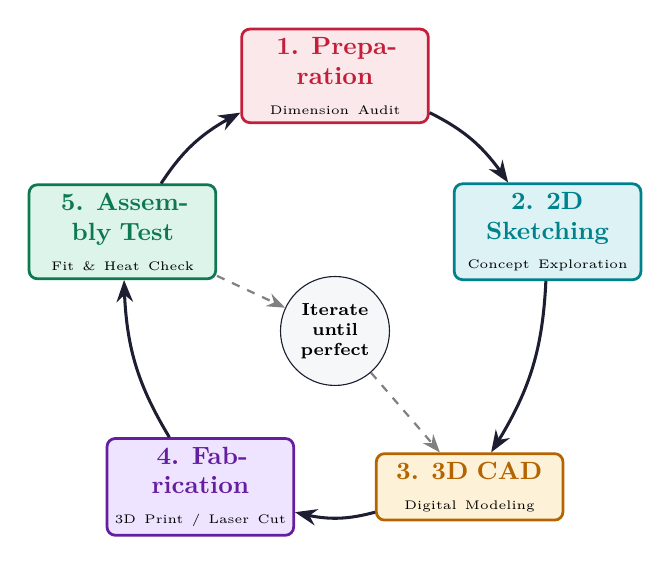
\begin{tikzpicture}[scale=0.9, transform shape]
  % Nodes in a loop (Enlarged coordinates to prevent collision)
  \node[draw=myred, fill=hdrred, rounded corners=3pt, line width=1pt, text width=2.4cm, align=center, minimum height=0.9cm] (prep) at (0, 3.2) {
    \textbf{\color{myred}1. Preparation}\\
    \tiny Dimension Audit
  };

  \node[draw=myteal, fill=hdrteal, rounded corners=3pt, line width=1pt, text width=2.4cm, align=center, minimum height=0.9cm] (sketch) at (3.0, 1.0) {
    \textbf{\color{myteal}2. 2D Sketching}\\
    \tiny Concept Exploration
  };

  \node[draw=myamber, fill=hdramber, rounded corners=3pt, line width=1pt, text width=2.4cm, align=center, minimum height=0.9cm] (cad) at (1.9, -2.6) {
    \textbf{\color{myamber}3. 3D CAD}\\
    \tiny Digital Modeling
  };

  \node[draw=mypurple, fill=hdrpurple, rounded corners=3pt, line width=1pt, text width=2.4cm, align=center, minimum height=0.9cm] (fab) at (-1.9, -2.6) {
    \textbf{\color{mypurple}4. Fabrication}\\
    \tiny 3D Print / Laser Cut
  };

  \node[draw=mygreen, fill=hdrgreen, rounded corners=3pt, line width=1pt, text width=2.4cm, align=center, minimum height=0.9cm] (test) at (-3.0, 1.0) {
    \textbf{\color{mygreen}5. Assembly Test}\\
    \tiny Fit \& Heat Check
  };

  % Loop Arrows
  \draw[arrow, bend left=15, line width=1.1pt] (prep) to (sketch);
  \draw[arrow, bend left=15, line width=1.1pt] (sketch) to (cad);
  \draw[arrow, bend left=15, line width=1.1pt] (cad) to (fab);
  \draw[arrow, bend left=15, line width=1.1pt] (fab) to (test);
  \draw[arrow, bend left=15, line width=1.1pt] (test) to (prep);

  % Central node
  \node[draw=mydark, fill=mygray, circle, inner sep=3pt, font=\scriptsize\bfseries, align=center] (center) at (0, -0.4) {Iterate\\until\\perfect};
  
  \draw[arrow, dashed, color=gray] (test) -- (center);
  \draw[arrow, dashed, color=gray] (center) -- (cad);
\end{tikzpicture}
\end{tcolorbox}

% ===============================================================================
\section{Prototyping Methods}
% ===============================================================================

Various low-fidelity and high-fidelity fabrication methods are used depending on the design stage.

\subsection{Non-Digital Prototyping (Low-Fidelity)}
Before using digital machines, designers build fast, manual models using cardboard, foam core, acrylic sheets, and modeling clay.
\begin{itemize}[leftmargin=*, itemsep=2.5pt]
  \item \textbf{Advantages:} Extremely low cost, zero machine wait time, and allows testing basic dimensions in a few minutes.
  \item \textbf{Drawback:} Low precision, fragile, and cannot be used for mechanical testing.
\end{itemize}

\subsection{Laser Cutting (2D Vector Fabrication)}
Laser cutting uses a high-power laser beam to cut or engrave sheet materials (acrylic, MDF, plywood, cardboard) based on 2D vector drawing profiles.
\begin{itemize}[leftmargin=*, itemsep=3.5pt]
  \item \textbf{Vector Layouts:} Drawn in programs like Inkscape or AutoCAD using closed paths.
  \item \textbf{Kerf:} The width of the material that is vaporized by the laser beam during cutting (typically $0.1\text{mm}$ to $0.3\text{mm}$). To create tight press-fit or finger joints, the design dimensions must compensate for this kerf allowance.
  \item \textbf{Joint Assembly Types:}
        \begin{itemize}[leftmargin=*, label=$\circ$, itemsep=1.0pt]
          \item \textit{Finger/Box Joints:} Interlocking rectangular teeth along edges, glued or press-fit.
          \item \textit{T-Slot Joints:} A slot receives a nut, and a perpendicular screw pulls the interlocking face tight. Excellent for structures needing frequent disassembly.
          \item \textit{Mortise and Tenon:} A tab (tenon) fits tightly into a matching slot (mortise) to align panels.
        \end{itemize}
\end{itemize}

\subsection{3D Printing (Additive Manufacturing)}
\begin{tcolorbox}[defbox, title={3D Printing (Additive)}]
  \textbf{3D Printing} is an additive manufacturing process that builds 3D solid structures layer-by-layer from a digital CAD file. The dominant technology is \textbf{FDM (Fused Deposition Modeling)}, which extrudes molten thermoplastic filament (PLA, ABS) through a heated nozzle.
\end{tcolorbox}
Key 3D printing parameters that affect enclosure durability and print time:
\begin{itemize}[leftmargin=*, itemsep=3pt]
  \item \textbf{Layer Height:} Controls vertical resolution (typically $0.1\text{mm}$ to $0.3\text{mm}$). Smaller values give smoother surfaces but increase print time.
  \item \textbf{Infill Density \& Patterns:} The internal grid structure, ranging from $0\%$ (hollow) to $100\%$ (solid). Enclosures typically use $15\%$ to $30\%$ infill. Patterns include \textit{Honeycomb} (strongest in multiple axes), \textit{Gyroid} (isometric strength and flexibility), and \textit{Grid} (fastest printing).
  \item \textbf{Wall/Shell Thickness:} The thickness of the outer boundaries, defining enclosure strength and screw-mounting thread durability.
  \item \textbf{Materials:}
        \begin{itemize}[leftmargin=*, label=$\circ$, itemsep=1.0pt]
          \item \textit{PLA (Polylactic Acid):} Biodegradable starch-based polymer. Easy to print, low warping, but low temperature resistance (warps above $60^\circ\text{C}$).
          \item \textit{ABS (Acrylonitrile Butadiene Styrene):} Petroleum-based. Highly impact-resistant, high heat deflection, but requires a heated enclosure and emits toxic fumes during printing.
          \item \textit{PETG (Polyethylene Terephthalate Glycol):} Blends ease of PLA with durability of ABS. Excellent chemical and weather resistance, ideal for outdoor IoT nodes.
        \end{itemize}
\end{itemize}

\subsection{CNC Milling (Subtractive Manufacturing)}
CNC (Computer Numerical Control) milling uses rotating cutting bits to carve away material from a solid block of plastic, wood, or metal (aluminum).
\begin{itemize}[leftmargin=*, itemsep=3pt]
  \item \textbf{Subtractive Concept:} The opposite of 3D printing. It starts with a solid stock block and subtracts material using high-speed rotary cutters.
  \item \textbf{Milling Toolpaths:} G-code instructions define specific cutter movements:
        \begin{itemize}[leftmargin=*, label=$\circ$, itemsep=1.0pt]
          \item \textit{Pocketing:} Carving out internal hollow cavities inside a solid block (e.g. creating the box cavity for electronics).
          \item \textit{Contouring (Profiling):} Cutting along outer boundary lines to separate the final piece from raw stock.
          \item \textit{Facing:} Machining flat surfaces on a block to ensure absolute thickness tolerance.
        \end{itemize}
  \item \textbf{Applications:} Best for high-strength enclosures, metal heat-sink cases, and prototyping circuit boards (PCB isolation routing).
\end{itemize}

\subsection{Repurposing and Recycling}
Hacking off-the-shelf plastic junction boxes, containers, or toys by drilling holes for cables and sensors.
\begin{itemize}[leftmargin=*, itemsep=2.5pt]
  \item \textbf{Advantages:} Provides immediate structural protection, is highly cost-effective, and reduces e-waste footprint during research stages.
\end{itemize}

\newpage

% ═══════════════════════════════════════════════════════════════════════════════
% QUICK REVISION PAGE
% ═══════════════════════════════════════════════════════════════════════════════
\begin{center}
  {\large\bfseries\color{myred} Quick Revision — Module 4}\\[3pt]
  {\small\color{mydark} Physical Design \& Prototyping $|$ OE-EC803A}
\end{center}
\noindent{\color{myred}\rule{\linewidth}{1.2pt}}
\vspace{8pt}

\begin{tcolorbox}[defbox, title={\textbf{One-Line Definitions}}]
\begin{itemize}[leftmargin=*, itemsep=3pt, topsep=0pt]
  \item \textbf{Kerf:} The thickness of the cut line or material slot vaporized by a laser cutter.
  \item \textbf{FDM:} A 3D printing process that builds objects by extruding layers of melted plastic filament.
  \item \textbf{Subtractive Manufacturing:} A fabrication process where material is carved away from a solid block.
  \item \textbf{Additive Manufacturing:} A fabrication process where material is joined layer-by-layer to build a structure.
  \item \textbf{Infill:} The internal supporting pattern printed inside a 3D object to save time and material.
\end{itemize}
\tcblower
Understanding the kerf is critical for press-fit joints where interlocking teeth must hold together without glue.
\end{tcolorbox}

\vspace{6pt}

\begin{tcolorbox}[exambox, title={\textbf{Frequently Asked / Viva Questions}}]
\begin{enumerate}[leftmargin=*, topsep=0pt, label=\textbf{Q\arabic*.}, itemsep=6pt]
  \item \Q{What is the difference between additive and subtractive manufacturing?}
        Additive manufacturing (e.g. 3D printing) builds parts layer-by-layer from nothing, producing zero waste and allowing complex internal cavities. Subtractive manufacturing (e.g. CNC milling) carves parts out of a solid block of raw material, producing waste chips but yielding high strength and support for metals.
        
  \item \Q{Explain the significance of ``kerf'' in laser cutting.}
        The kerf is the width of the cut slot created by the laser beam vaporizing material. If a laser has a kerf of $0.2\text{mm}$, cutting a $10.0\text{mm}$ square will result in a piece that is $9.8\text{mm}$ wide. Designers must compensate for this kerf to create tight, interlocking press-fit joints.
        
  \item \Q{Why is infill density in 3D printing rarely set to $100\%$?}
        A $100\%$ infill uses massive amounts of filament and takes a very long time to print. Structural strength gains level off significantly beyond $40\%$ infill. Enclosures are usually printed with $15\%$ to $30\%$ infill using internal patterns (like grid or gyroid) to maximize strength-to-weight ratio.
        
  \item \Q{What is Fused Deposition Modeling (FDM)?}
        FDM is the most common 3D printing technology. It melts a plastic filament (like PLA or ABS) and extrudes it through a small nozzle, moving in X, Y, and Z axes to lay down thin layers that fuse together as they cool.
        
  \item \Q{Why would a designer choose CNC milling over 3D printing for an industrial IoT gateway enclosure?}
        CNC milling allows using materials like structural aluminum. Aluminum enclosures provide superior mechanical protection, complete electromagnetic shielding (Faraday cage), and act as built-in heat sinks for high-power processors.
        
  \item \Q{What is the purpose of low-fidelity physical prototyping using cardboard?}
        Low-fidelity prototyping allows designers to physically hold and check the dimensions of a device layout within minutes, helping catch major interface errors (like port placement blockage or button hand-reach issues) before executing expensive machine runs.
        
  \item \Q{What is repurposing/recycling in physical design?}
        Repurposing refers to taking an existing mass-produced plastic box (like an electrical junction box or soap container) and drilling custom ports to house the IoT circuit. This saves cost, is weather-sealed, and reduces development time.
        
  \item \Q{What is SLA (Stereolithography) 3D printing, and how does it differ from FDM?}
        SLA uses a liquid photopolymer resin that is cured layer-by-layer using a UV laser beam. It yields extremely high resolutions and smooth surface finishes compared to FDM, but the materials are more fragile and require post-print chemical cleaning.
\end{enumerate}
\end{tcolorbox}

\vspace{6pt}

\begin{tcolorbox}[tikzbox, title={\textbf{Comparison Snapshot}}]
\textbf{3D Printing vs. CNC Milling vs. Laser Cutting:}\par\vspace{6pt}\noindent
{\renewcommand{\arraystretch}{1.35}%
\begin{tabularx}{\linewidth}{|B{3.2cm}|Y|Y|Y|}
\hline
\textbf{Feature} & \textbf{3D Printing (FDM)} & \textbf{CNC Milling} & \textbf{Laser Cutting} \\
\hline
Process & Additive (layer-by-layer). & Subtractive (carving). & 2D Cutting / Engraving. \\
\hline
Dimensions & Complex 3D geometries. & 3D shapes with tool limitations. & Flat 2D sheets (can fold/slot). \\
\hline
Materials & PLA, ABS, PETG. & Metals (Al, Steel), Wood, Acetal. & Acrylic, MDF, Plywood, Cardboard. \\
\hline
Wastage & Very Low (only support material). & High (residual chips and dust). & Low-Medium (sheet offcuts). \\
\hline
Setup Speed & Very Fast (load STL to printer). & Slow (requires CAM setups, tools). & Fast (load vector file). \\
\hline
\end{tabularx}}
\end{tcolorbox}


% -- Module 5 -----------------------------------------------------------------
\modulestart{5}{Prototyping Online Components (APIs)}

\section{Prototyping Online Components (APIs)}
% ===============================================================================

To connect physical hardware to cloud services, devices communicate with web application interfaces called APIs (Application Programming Interfaces).

\subsection{RESTful APIs}
\begin{tcolorbox}[defbox, title={REST API}]
  A \textbf{REST (Representational State Transfer) API} is an architectural style for network applications that uses standard HTTP requests to manage resources. Each resource is identified by a URL (e.g. `/devices/lamp1`) and manipulated using standard HTTP verbs.
\end{tcolorbox}
The primary HTTP verbs used in IoT APIs include:
\begin{itemize}[leftmargin=*, itemsep=2pt]
  \item \textbf{GET:} Retrieve the status/value of a sensor or actuator.
  \item \textbf{POST:} Create a new status log or register a new device.
  \item \textbf{PUT / PATCH:} Update configuration properties or toggle state.
  \item \textbf{DELETE:} Remove a device instance from the registry database.
\end{itemize}

Common HTTP response status codes returned by IoT APIs:
\begin{itemize}[leftmargin=*, itemsep=2.5pt]
  \item \textbf{200 OK:} Request succeeded (e.g. GET returned sensor reading).
  \item \textbf{201 Created:} Resource successfully created (e.g. POST registered a new device).
  \item \textbf{400 Bad Request:} Invalid syntax or malformed JSON payload.
  \item \textbf{401 Unauthorized:} Missing or invalid API key / authentication token.
  \item \textbf{404 Not Found:} Target device or resource URL does not exist.
  \item \textbf{500 Internal Server Error:} Server-side runtime database/connection failure.
\end{itemize}

Data is commonly formatted in \textbf{JSON (JavaScript Object Notation)} due to its low parsing overhead and human-readable, key-value structure:
\begin{verbatim}
{
  "device_id": "sensor_node_04",
  "temperature": 26.5,
  "status": "active"
}
\end{verbatim}
\subsection{Writing a New API (Backend Endpoint)}
Writing a new REST API endpoint involves setting up a server runtime (e.g. Node.js with Express or Python with Flask) that accepts incoming JSON payloads, processes them, and returns standard HTTP response codes.
\begin{tcolorbox}[examplebox, title={Express.js IoT Server-Side Logging API}]
  Below is a standard server-side Node.js script that listens for HTTP \texttt{POST} requests from IoT sensor nodes and saves the reading:
\begin{verbatim}
const express = require('express');
const app = express();
app.use(express.json()); // Parse JSON payloads

app.post('/api/telemetry', (req, res) => {
  const { device_id, temperature } = req.body;
  
  if (!device_id || temperature === undefined) {
    return res.status(400).json({ error: "Missing parameters" });
  }
  
  console.log(`Log from ${device_id}: ${temperature} C`);
  // (In production: Insert data into MongoDB or PostgreSQL database)
  
  res.status(201).json({ 
    message: "Data logged successfully", 
    timestamp: new Date() 
  });
});

app.listen(3000, () => console.log('IoT Server running on port 3000'));
\end{verbatim}
\end{tcolorbox}
\subsection{Real-Time Reactions: Polling vs. WebSockets}
IoT systems need to push real-time events (e.g., triggering an alarm).
\begin{itemize}[leftmargin=*, itemsep=3.5pt]
  \item \textbf{HTTP Polling:} The client periodically sends GET requests to the server (e.g., every 5 seconds) to check for updates. This generates significant network overhead and latency.
  \item \textbf{HTTP Long Polling:} The server holds the client's request open until new data is available, responding immediately, then closing the connection.
  \item \textbf{WebSockets:} Establishes a persistent, bi-directional TCP connection. Both client and server can send data packets at any time with minimal header overhead, enabling sub-millisecond real-time reactions.
\end{itemize}

\begin{tcolorbox}[tikzbox, title={HTTP Polling vs. WebSockets Communication Flow}]
\centering
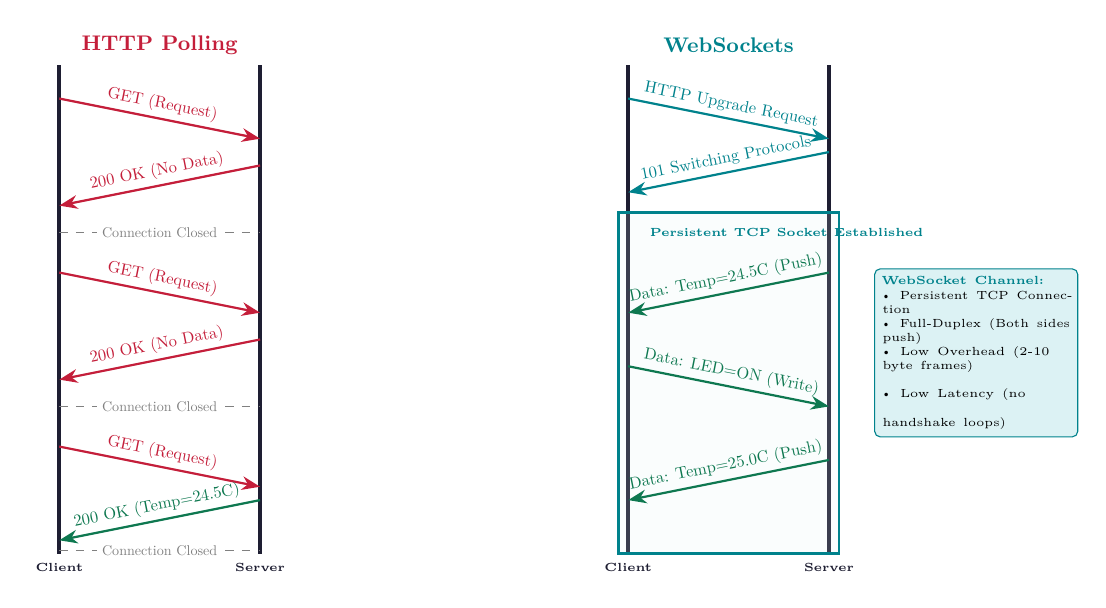
\begin{tikzpicture}[scale=0.85, transform shape]
  % ═══════════════════════════════════════════════════════════════════════════════
  % LEFT SIDE: HTTP POLLING (Wider spacing, sloped text labels)
  % ═══════════════════════════════════════════════════════════════════════════════
  \node[font=\small\bfseries\color{myred}] at (-6.0, 3.8) {HTTP Polling};
  \draw[line width=1.5pt, color=mydark] (-7.5, 3.5) -- (-7.5, -3.8) node[below, font=\tiny\bfseries] {Client};
  \draw[line width=1.5pt, color=mydark] (-4.5, 3.5) -- (-4.5, -3.8) node[below, font=\tiny\bfseries] {Server};

  % Exchange 1
  \draw[arrow, color=myred] (-7.5, 3.0) -- node[midway, above, sloped, scale=0.7] {GET (Request)} (-4.5, 2.4);
  \draw[arrow, color=myred] (-4.5, 2.0) -- node[midway, above, sloped, scale=0.7] {200 OK (No Data)} (-7.5, 1.4);
  \draw[dashed, color=gray] (-7.5, 1.0) -- (-4.5, 1.0) node[midway, fill=white, scale=0.6] {Connection Closed};

  % Exchange 2
  \draw[arrow, color=myred] (-7.5, 0.4) -- node[midway, above, sloped, scale=0.7] {GET (Request)} (-4.5, -0.2);
  \draw[arrow, color=myred] (-4.5, -0.6) -- node[midway, above, sloped, scale=0.7] {200 OK (No Data)} (-7.5, -1.2);
  \draw[dashed, color=gray] (-7.5, -1.6) -- (-4.5, -1.6) node[midway, fill=white, scale=0.6] {Connection Closed};

  % Exchange 3
  \draw[arrow, color=myred] (-7.5, -2.2) -- node[midway, above, sloped, scale=0.7] {GET (Request)} (-4.5, -2.8);
  \draw[arrow, color=mygreen] (-4.5, -3.0) -- node[midway, above, sloped, scale=0.7] {200 OK (Temp=24.5C)} (-7.5, -3.6);
  \draw[dashed, color=gray] (-7.5, -3.75) -- (-4.5, -3.75) node[midway, fill=white, scale=0.6] {Connection Closed};


  % ═══════════════════════════════════════════════════════════════════════════════
  % RIGHT SIDE: WEBSOCKETS (Wider spacing, side-aligned description box)
  % ═══════════════════════════════════════════════════════════════════════════════
  \node[font=\small\bfseries\color{myteal}] at (2.5, 3.8) {WebSockets};
  \draw[line width=1.5pt, color=mydark] (1.0, 3.5) -- (1.0, -3.8) node[below, font=\tiny\bfseries] {Client};
  \draw[line width=1.5pt, color=mydark] (4.0, 3.5) -- (4.0, -3.8) node[below, font=\tiny\bfseries] {Server};

  % Handshake (HTTP Upgrade)
  \draw[arrow, color=myteal] (1.0, 3.0) -- node[midway, above, sloped, scale=0.7] {HTTP Upgrade Request} (4.0, 2.4);
  \draw[arrow, color=myteal] (4.0, 2.2) -- node[midway, above, sloped, scale=0.7] {101 Switching Protocols} (1.0, 1.6);

  % Persistent Connection Channel Box
  \draw[draw=myteal, fill=hdrteal, fill opacity=0.15, line width=1pt] (0.85, 1.3) rectangle (4.15, -3.8);
  \node[right, font=\tiny\bfseries, color=myteal] at (1.2, 1.0) {Persistent TCP Socket Established};

  % Bidirectional Pushes
  \draw[arrow, color=mygreen] (4.0, 0.4) -- node[midway, above, sloped, scale=0.7] {Data: Temp=24.5C (Push)} (1.0, -0.2);
  \draw[arrow, color=mygreen] (1.0, -1.0) -- node[midway, above, sloped, scale=0.7] {Data: LED=ON (Write)} (4.0, -1.6);
  \draw[arrow, color=mygreen] (4.0, -2.4) -- node[midway, above, sloped, scale=0.7] {Data: Temp=25.0C (Push)} (1.0, -3.0);

  % WebSocket Features Box (Placed completely to the right to prevent overlap)
  \node[draw=myteal, fill=hdrteal, rounded corners=2pt, text width=2.8cm, align=left] at (6.2, -0.8) {
    \tiny
    \textbf{\color{myteal}WebSocket Channel:}\\
    • Persistent TCP Connection\\
    • Full-Duplex (Both sides push)\\
    • Low Overhead (2-10 byte frames)\\
    • Low Latency (no handshake loops)
  };
\end{tikzpicture}
\end{tcolorbox}

\subsection{Other Messaging Protocols}
\begin{itemize}[leftmargin=*, itemsep=2.5pt]
  \item \textbf{XMPP (Extensible Messaging and Presence Protocol):} XML-based instant messaging protocol. Heavy overhead but features strong built-in security and routing.
  \item \textbf{AMQP (Advanced Message Queuing Protocol):} An open standard queuing protocol designed for enterprise transaction messaging, providing high reliability.
\end{itemize}

% ===============================================================================
\section{Techniques for Writing Embedded Code}
% ===============================================================================

Microcontrollers are resource-constrained devices, requiring specialized programming practices.

\subsection{Memory Management \& Heap Fragmentation}
\begin{tcolorbox}[defbox, title={Heap Fragmentation}]
  \textbf{Heap Fragmentation} occurs when dynamic memory allocation (`malloc()` and `free()`) allocates and deallocates varying memory chunks over time, leaving small, unusable gaps in the heap. In microcontrollers with only a few kilobytes of RAM, this can eventually prevent large allocations, leading to program crashes.
\end{tcolorbox}
To prevent fragmentation, embedded code should:
\begin{itemize}[leftmargin=*, itemsep=2.5pt]
  \item Avoid dynamic memory (`new`, `malloc`, `String` objects).
  \item Prefer static global allocation (defining buffer arrays with fixed sizes at compile time) or stack-based local variables.
\end{itemize}

\subsection{Power Management and Battery Life Optimization}
Many IoT devices run on batteries, requiring strict power management:
\begin{itemize}[leftmargin=*, itemsep=3pt]
  \item \textbf{Active Mode:} CPU running at full clock speed, radio transmitting. Draws high current ($10\text{mA}$ to $150\text{mA}$).
  \item \textbf{Light Sleep:} CPU clock is gated/halted, RAM is preserved. Draws microamps ($100\mu\text{A}$ to $500\mu\text{A}$).
  \item \textbf{Deep Sleep:} CPU, RAM, and internal oscillators are completely shut down. Only an ultra-low-power Real-Time Clock (RTC) or external interrupt remains active. Draws nanoamps ($1\mu\text{A}$ to $15\mu\text{A}$). The device wakes up, reads sensors, transmits, and immediately sleeps again.
\end{itemize}

\begin{tcolorbox}[formulabox, title={Duty Cycling \& Battery Life}]
  \textbf{Duty Cycling} is the ratio of active time ($t_{\text{active}}$) to the total period ($T = t_{\text{active}} + t_{\text{sleep}}$):
  \begin{equation}
    D = \frac{t_{\text{active}}}{t_{\text{active}} + t_{\text{sleep}}}
  \end{equation}
  The average current draw ($I_{\text{avg}}$) is calculated as:
  \begin{equation}
    I_{\text{avg}} = D \cdot I_{\text{active}} + (1 - D) \cdot I_{\text{sleep}}
  \end{equation}
  Battery lifetime ($L$ in hours) for a battery with capacity $C$ (in mAh) is:
  \begin{equation}
    L = \frac{C}{I_{\text{avg}}}
  \end{equation}
\end{tcolorbox}

\begin{tcolorbox}[examplebox, title={Numerical Example: IoT Battery Life Calculation}]
  \textbf{Scenario:} An IoT sensor node wakes up once every $10$ minutes ($600\text{ seconds}$) for a duration of $2\text{ seconds}$ to read a sensor and transmit it via Wi-Fi.
  \begin{itemize}[leftmargin=*, itemsep=2.5pt]
    \item Active Current ($I_{\text{active}}$) = $80\text{ mA}$
    \item Sleep Current ($I_{\text{sleep}}$) = $15\ \mu\text{A} = 0.015\text{ mA}$
    \item Battery Capacity ($C$) = $2400\text{ mAh}$ (e.g. standard AA cells)
  \end{itemize}
  \textbf{Step 1: Calculate Duty Cycle ($D$)}
  \begin{equation}
    D = \frac{2\text{ s}}{600\text{ s}} = 0.00333\quad (0.33\%)
  \end{equation}
  \textbf{Step 2: Calculate Average Current ($I_{\text{avg}}$)}
  \begin{equation}
    I_{\text{avg}} = (0.00333 \cdot 80\text{ mA}) + ((1 - 0.00333) \cdot 0.015\text{ mA})
  \end{equation}
  \begin{equation}
    I_{\text{avg}} \approx 0.2667\text{ mA} + 0.0150\text{ mA} = 0.2817\text{ mA}
  \end{equation}
  \textbf{Step 3: Calculate Battery Lifetime ($L$)}
  \begin{equation}
    L = \frac{2400\text{ mAh}}{0.2817\text{ mA}} \approx 8519.7\text{ hours} \approx 355\text{ days}
  \end{equation}
  Thus, by employing aggressive duty cycling, a standard battery can sustain the node for approximately one full year despite its high $80\text{mA}$ active transmission current.
\end{tcolorbox}

\subsection{Embedded Debugging Techniques}
Debugging on microcontrollers is challenging because they lack screens.
\begin{itemize}[leftmargin=*, itemsep=3pt]
  \item \textbf{Serial Debugging:} Printing variable values to a host computer serial monitor (`Serial.println()`). Simple but introduces delay (timing bugs).
  \item \textbf{In-Circuit Emulation \& JTAG:} A hardware interface (Joint Test Action Group) that connects directly to the CPU core, allowing developers to set hardware breakpoints, inspect memory registers, and step through code line-by-line.
\end{itemize}

\newpage

% ═══════════════════════════════════════════════════════════════════════════════
% QUICK REVISION PAGE
% ═══════════════════════════════════════════════════════════════════════════════
\begin{center}
  {\large\bfseries\color{myred} Quick Revision — Module 5}\\[3pt]
  {\small\color{mydark} Online Components \& Embedded Programming $|$ OE-EC803A}
\end{center}
\noindent{\color{myred}\rule{\linewidth}{1.2pt}}
\vspace{8pt}

\begin{tcolorbox}[formulabox, title={\textbf{Key Formulas and Metrics at a Glance}}]
\renewcommand{\arraystretch}{1.35}
\begin{tabularx}{\linewidth}{B{5.0cm} X}
  Duty Cycle & $D = \dfrac{t_{\text{active}}}{t_{\text{active}} + t_{\text{sleep}}} \quad (\text{ratio of active execution time})$ \\[4pt]
  Average Current & $I_{\text{avg}} = D \cdot I_{\text{active}} + (1 - D) \cdot I_{\text{sleep}} \quad (\text{power profile})$ \\[4pt]
  Battery Lifetime & $L = \dfrac{\text{Battery Capacity (mAh)}}{I_{\text{avg}} \text{ (mA)}} \quad (\text{operation hours})$
\end{tabularx}
\end{tcolorbox}

\vspace{6pt}

\begin{tcolorbox}[defbox, title={\textbf{One-Line Definitions}}]
\begin{itemize}[leftmargin=*, itemsep=3pt, topsep=0pt]
  \item \textbf{REST:} A stateless web architectural style that relies on standard HTTP methods (GET/POST).
  \item \textbf{WebSocket:} A persistent, full-duplex TCP socket connection for real-time web communication.
  \item \textbf{Duty Cycling:} The practice of powering down the device CPU and radio for periodic sleep intervals.
  \item \textbf{Deep Sleep:} The lowest power state of an MCU, turning off all internal blocks except the RTC wakeup timer.
  \item \textbf{JTAG:} A hardware port standard used for direct in-circuit programming, testing, and debugging.
\end{itemize}
\end{tcolorbox}

\vspace{6pt}

\begin{tcolorbox}[exambox, title={\textbf{Frequently Asked / Viva Questions}}]
\begin{enumerate}[leftmargin=*, topsep=0pt, label=\textbf{Q\arabic*.}, itemsep=6pt]
  \item \Q{Why is dynamic memory allocation (`malloc`) highly discouraged in microcontroller code?}
        Microcontrollers have extremely limited RAM (often a few kilobytes) and no virtual memory management. Repeated allocations and deallocations leave small gaps of unused memory on the heap (heap fragmentation). Eventually, a request for a contiguous memory block fails, causing a system crash.
        
  \item \Q{Compare HTTP Polling and WebSockets for real-time sensor updates.}
        HTTP Polling requires the client to repeatedly send new request handshakes and headers, creating heavy network congestion and latency. WebSockets establishes a single persistent TCP connection, enabling bi-directional, real-time message streams with minimal packet overhead.
        
  \item \Q{Calculate the average current and battery life of an IoT node with a $1000\text{mAh}$ battery. It draws $100\text{mA}$ for $2$ seconds when active, and $10\mu\text{A}$ ($0.01\text{mA}$) for $58$ seconds during sleep.}
        (1) Total Period $T = 2 + 58 = 60$ seconds. (2) Duty Cycle $D = 2 / 60 = 0.0333$ ($3.33\%$). (3) Average Current $I_{\text{avg}} = (0.0333 \times 100) + (0.9667 \times 0.01) = 3.33 + 0.0097 \approx 3.34\text{mA}$. (4) Lifetime $L = 1000 / 3.34 \approx 299.4$ hours ($\approx 12.5$ days).
        
  \item \Q{What occurs during deep sleep in an ESP8266 or ESP32 microcontroller?}
        During deep sleep, the CPU, RAM, and internal Wi-Fi radio are completely powered off. The only part of the chip that remains powered is the low-power RTC timer and select GPIO wake pins. The CPU must re-initialize (reboot) from scratch when waking up.
        
  \item \Q{What is a REST API HTTP POST request used for in IoT?}
        A POST request is used to push data from the client to the server, creating a new database record (e.g., posting a new temperature reading log at `/api/v1/telemetry`).
        
  \item \Q{Explain the JTAG debug interface.}
        JTAG is a hardware debugging protocol. It uses dedicated physical pins on the microcontroller to interface directly with the internal processor tap, allowing developers to halt CPU execution, step through commands, and read register states.
        
  \item \Q{What is JSON, and why is it preferred over XML in IoT applications?}
        JSON is a lightweight key-value text format for representing structured data. It has a much smaller character count than XML (no closing tags), which saves bandwidth, and requires significantly less CPU memory and time to parse.
        
  \item \Q{How does duty cycling extend device battery life?}
        Sensors rarely need to transmit data continuously. By sleeping for $99\%$ of the time and only waking up for a few seconds to sample and transmit data, the average current draw is reduced to microamps, extending battery life from days to years.
\end{enumerate}
\end{tcolorbox}

\vspace{6pt}

\begin{tcolorbox}[tikzbox, title={\textbf{Comparison Snapshot}}]
\textbf{HTTP Polling vs. WebSockets:}\par\vspace{6pt}\noindent
{\renewcommand{\arraystretch}{1.35}%
\begin{tabularx}{\linewidth}{|B{3.2cm}|Y|Y|}
\hline
\textbf{Feature} & \textbf{HTTP Polling} & \textbf{WebSockets} \\
\hline
Connection Type & Temporary; opened and closed per request. & Persistent; remains open until closed. \\
\hline
Communication & Half-duplex (client pull only). & Full-duplex (bi-directional push/pull). \\
\hline
Network Overhead & High (repeats TCP handshakes and HTTP headers). & Minimal (small frame header of 2-10 bytes). \\
\hline
Real-Time Latency & High (depends on polling frequency). & Extremely Low (sub-millisecond). \\
\hline
Best Use Case & Static data dashboards. & Real-time alerts, remote live control. \\
\hline
\end{tabularx}}
\end{tcolorbox}


% -- Module 6 -----------------------------------------------------------------
\modulestart{6}{IoT Business Models \& Startups}

\section{IoT Business Models \& Startups}
% ===============================================================================

Transitioning an IoT prototype into a commercial product requires establishing sustainable business value.

\subsection{A Short History of Business Models}
Historically, business models revolved around the \textbf{transactional model} (Value-Transaction-Exchange), where companies designed, manufactured, and sold physical products as a one-time purchase. 
In the digital age, this evolved into the \textbf{subscription/service-based model} (e.g. SaaS). IoT merges these two histories: it combines the transactional sale of physical hardware with the ongoing subscription-based service model (Product-as-a-Service), creating a continuous customer relationship.

\subsection{Who is the Business Model For?}
An IoT business model serves three main target audiences:
\begin{itemize}[leftmargin=*, itemsep=3.0pt]
  \item \textbf{Investors:} Demonstrates the viability, return on investment (ROI), scalability, and path to profitability (amortizing high upfront tooling and NRE costs).
  \item \textbf{Partners and Suppliers:} Clarifies roles in the value chain, such as PCB manufacturing houses, cloud providers, and distribution networks.
  \item \textbf{Internal Team:} Aligns the engineering, sales, and support departments on customer needs, product value propositions, and resource allocations.
\end{itemize}

\subsection{Business Model Canvas in IoT}
The \textbf{Business Model Canvas} defines a startup's value chain across 9 building blocks. IoT products alter these blocks:
\begin{enumerate}[leftmargin=*, itemsep=3.0pt]
  \item \textbf{Value Proposition:} Continuous software updates, predictive maintenance, and remote automation rather than just static physical utility.
  \item \textbf{Revenue Streams:} Low upfront hardware margins compensated by recurring subscription models (SaaS / Hardware-as-a-Service).
  \item \textbf{Customer Segments:} Distinct B2C (consumers desiring convenience) vs. B2B (enterprises desiring efficiency/analytics).
  \item \textbf{Customer Relationships:} Continuous digital engagement via apps and automated support, rather than one-time transaction endpoints.
  \item \textbf{Channels:} Digital app stores and direct e-commerce, paired with physical retail and distribution channels.
  \item \textbf{Key Activities:} Firmware maintenance, OTA software updates, security patch deployment, and cloud server scaling.
  \item \textbf{Key Resources:} Proprietary sensor algorithms, cloud database infrastructure, engineering talent, and manufacturing supply chains.
  \item \textbf{Key Partners:} Cloud platform providers (AWS, Azure), silicon chip vendors, contract manufacturers, and network carrier operators.
  \item \textbf{Cost Structure:} High initial NRE (Non-Recurring Engineering) tooling costs, bill of materials (BOM), cloud bandwidth, and continuous server hosting costs.
\end{enumerate}

\subsection{Lean Startup Methodology}
\begin{itemize}[leftmargin=*, itemsep=3pt]
  \item \textbf{MVP (Minimum Viable Product):} Building a prototype containing only the core feature that solves the user's primary problem.
  \item \textbf{Feedback Loop:} The iterative \textbf{Build-Measure-Learn} loop helps refine the MVP based on real user feedback before funding expensive manufacturing tooling.
\end{itemize}

\subsection{Funding Options}
IoT startups fund early stages via:
\begin{itemize}[leftmargin=*, itemsep=2pt]
  \item \textbf{Crowdfunding (Kickstarter):} Users pre-order the product, verifying market demand and funding initial production runs.
  \item \textbf{Venture Capital (VC) \& Bootstrapping:} Institutional funding for scaling versus self-funding from revenues.
\end{itemize}

% ===============================================================================
\section{Moving to Manufacture}
% ===============================================================================

Mass-producing electronic hardware involves transitioning from breadboards to industrial assembly lines.

\subsection{What are you Producing? \& Designing Kits}
Before manufacturing, developers must define the physical scope of their product:
\begin{itemize}[leftmargin=*, itemsep=3.0pt]
  \item \textbf{What are you Producing?:} Is the product a raw sub-assembly component, an industrial sensor node, or a polished end-user consumer product? This determines the enclosure design and target user experience.
  \item \textbf{Designing Kits:} Many IoT systems begin as developer kits (e.g. SparkFun/Adafruit starter kits). Designing a kit requires organizing components, color-coding wire connectors, providing clear assembly diagrams, and bundling software library links to reduce the user's first-time configuration friction.
\end{itemize}

\begin{tcolorbox}[tikzbox, title={IoT Product Development and Manufacturing Lifecycle}]
\centering
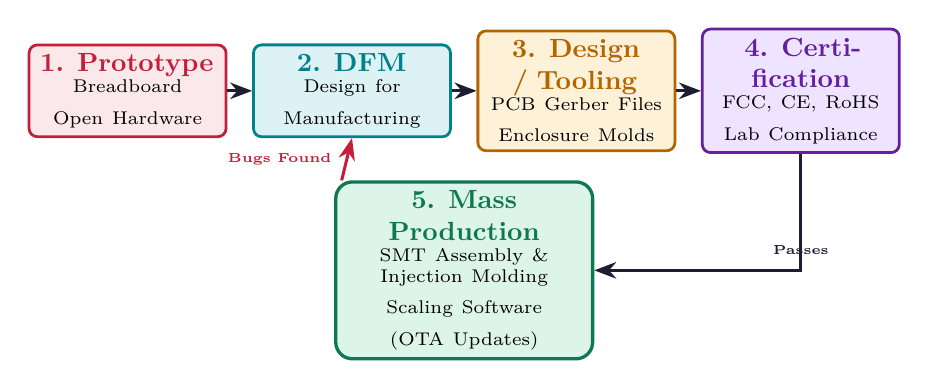
\begin{tikzpicture}[scale=0.95, transform shape]
  % Nodes
  \node[draw=myred, fill=hdrred, rounded corners=3pt, line width=1pt, text width=2.4cm, align=center, minimum height=1.1cm] (proto) at (-4.5, 0) {
    \textbf{\color{myred}1. Prototype}\\
    \scriptsize Breadboard\\
    \scriptsize Open Hardware
  };

  \node[draw=myteal, fill=hdrteal, rounded corners=3pt, line width=1pt, text width=2.4cm, align=center, minimum height=1.1cm] (dfm) at (-1.5, 0) {
    \textbf{\color{myteal}2. DFM}\\
    \scriptsize Design for\\
    \scriptsize Manufacturing
  };

  \node[draw=myamber, fill=hdramber, rounded corners=3pt, line width=1pt, text width=2.4cm, align=center, minimum height=1.1cm] (tool) at (1.5, 0) {
    \textbf{\color{myamber}3. Design / Tooling}\\
    \scriptsize PCB Gerber Files\\
    \scriptsize Enclosure Molds
  };

  \node[draw=mypurple, fill=hdrpurple, rounded corners=3pt, line width=1pt, text width=2.4cm, align=center, minimum height=1.1cm] (cert) at (4.5, 0) {
    \textbf{\color{mypurple}4. Certification}\\
    \scriptsize FCC, CE, RoHS\\
    \scriptsize Lab Compliance
  };

  \node[draw=mygreen, fill=hdrgreen, rounded corners=6pt, line width=1.2pt, text width=3.2cm, align=center, minimum height=1.2cm] (prod) at (0, -2.4) {
    \textbf{\color{mygreen}5. Mass Production}\\
    \scriptsize SMT Assembly \& Injection Molding\\
    \scriptsize Scaling Software (OTA Updates)
  };

  % Connections
  \draw[arrow, line width=1.1pt] (proto) -- (dfm);
  \draw[arrow, line width=1.1pt] (dfm) -- (tool);
  \draw[arrow, line width=1.1pt] (tool) -- (cert);
  
  % Passes arrow - enters prod.east horizontally from the right to avoid border-riding
  \draw[arrow, line width=1.1pt] (cert.south) |- node[midway, above=2pt, font=\tiny\bfseries] {Passes} (prod.east);
    
  % Bugs Found feedback loop - clean straight vertical line to dfm.south
  \draw[arrow, line width=1.1pt, color=myred] ($(prod.north west)+(0.1, 0)$) -- node[midway, left=2pt, font=\tiny\bfseries] {Bugs Found} (dfm.south);
\end{tikzpicture}
\end{tcolorbox}

\subsection{Designing and Manufacturing PCBs}
\begin{enumerate}[leftmargin=*, itemsep=4.0pt]
  \item \textbf{Schematic Capture:} Drawing the logical connectivity diagram between components using CAD software (e.g. KiCad, Altium).
  \item \textbf{PCB Layout Routing:} Arranging physical component footprints and routing copper traces to connect pins. Features include:
        \begin{itemize}[leftmargin=*, label=$\bullet$, itemsep=1.0pt]
          \item \textit{Trace Width:} Thicker traces are routed for power lines to handle current without overheating; thin traces are used for signals.
          \item \textit{Vias:} Plated copper cylinders that bridge traces between different layer planes.
          \item \textit{Ground Planes:} Large copper planes added to shield signals from EMI and provide a stable reference voltage.
        \end{itemize}
  \item \textbf{PCB Fabrication Steps:}
        \begin{itemize}[leftmargin=*, label=$\bullet$, itemsep=1.0pt]
          \item \textit{Etching:} Removing unwanted copper from substrate using chemical etchants (e.g. Ferric Chloride or Ammonium Persulfate).
          \item \textit{Drilling \& Electroplating:} Drilling mounting and via holes, then electroplating them with copper to establish layer connections.
          \item \textit{Solder Mask:} Applying a polymer layer (usually green) to insulate copper traces and prevent solder bridging.
          \item \textit{Surface Finish:} Coating exposed copper pads to prevent oxidation (e.g. \textbf{HASL} - Hot Air Solder Leveling, cheap; or \textbf{ENIG} - Electroless Nickel Immersion Gold, high-quality flat pads for fine SMT components).
        \end{itemize}
  \item \textbf{Assembly (SMT vs. Through-Hole):}
        \begin{itemize}[leftmargin=*, label=$\bullet$, itemsep=1pt]
          \item \textbf{SMT (Surface Mount Technology):} Components (SMD) are placed on solder paste and reflowed in an oven. Automated via pick-and-place machines; allows dual-sided, high-density designs.
          \item \textbf{Through-Hole Technology (THT):} Component pins are inserted through holes and wave-soldered. Essential for connectors and heavy power modules due to high mechanical strength.
        \end{itemize}
\end{enumerate}

\subsection{Mass-Producing Enclosures (Injection Molding)}
\begin{tcolorbox}[defbox, title={Injection Molding}]
  \textbf{Injection Molding} is the primary manufacturing process for plastic enclosures. Molten plastic (ABS, Polycarbonate) is injected under high pressure into a custom-machined steel or aluminum mold cavity, where it cools and solidifies into the final case.
\end{tcolorbox}
Key design constraints and manufacturing parameters for injection-molded parts:
\begin{itemize}[leftmargin=*, itemsep=3.0pt]
  \item \textbf{High Tooling Costs:} Machining the steel molds (tooling) is extremely expensive (often $\$10,000$ to $\$100,000$ NRE costs), requiring massive production volumes to amortize the setup cost.
  \item \textbf{Draft Angles:} Vertical walls must be tapered slightly (typically $1^\circ$ to $2^\circ$) to allow the solidified plastic part to eject easily from the steel mold without scratching.
  \item \textbf{Common Molding Defects:}
        \begin{itemize}[leftmargin=*, label=$\bullet$, itemsep=1.5pt]
          \item \textit{Sink Marks:} Shallow depressions formed on thick wall sections due to slower cooling and volumetric shrinkage. Fixed by maintaining uniform wall thickness.
          \item \textit{Warping:} Distortion of flat surfaces caused by non-uniform cooling rates across different sections of the part.
          \item \textit{Knit Lines (Weld Lines):} Lines where multiple molten plastic flow fronts meet and fail to fuse completely, representing structural weak spots.
          \item \textit{Flash:} Excess plastic leakage that escapes along the parting line of the mold halves due to low clamping pressure.
        \end{itemize}
\end{itemize}

\subsection{Hardware Certification}
Before selling electronic products, they must satisfy regulatory standards:
\begin{itemize}[leftmargin=*, itemsep=3.5pt]
  \item \textbf{FCC (Federal Communications Commission) Certification:} Required for products sold in the United States. It regulates electromagnetic compatibility (EMC):
        \begin{itemize}[leftmargin=*, label=$\bullet$, itemsep=1.0pt]
          \item \textit{Intentional Radiators:} Devices that actively broadcast RF signals (e.g. Wi-Fi, Bluetooth, cellular). Require full, expensive transmitter testing and registration.
          \item \textit{Unintentional Radiators:} Devices that do not intentionally broadcast radio signals but generate internal high-frequency signals ($>9\text{ kHz}$) like CPU clocks. Require self-declaration or verification.
        \end{itemize}
  \item \textbf{CE (Conformité Européenne) Marking:} Mandatory for products in the European Economic Area. Declares that the product complies with health, safety, and environmental protection directives (such as the Radio Equipment Directive - RED, and EMC Directive).
  \item \textbf{RoHS (Restriction of Hazardous Substances):} Restricts the use of specific hazardous substances in electrical and electronic equipment (specifically Lead, Mercury, Cadmium, Hexavalent Chromium, and flame retardants like PBB/PBDE). Requires lead-free solder and components.
\end{itemize}

\subsection{Manufacturing Cost Concepts}
Managing economics is critical when moving to mass manufacture:
\begin{itemize}[leftmargin=*, itemsep=3.5pt]
  \item \textbf{BOM (Bill of Materials):} A complete, hierarchical spreadsheet list of every raw component, IC, circuit board, enclosure part, connector, screw, and label required to manufacture one single unit, including supplier part numbers and cost-breaks.
  \item \textbf{NRE (Non-Recurring Engineering):} The one-time, upfront development cost of design, PCB routing labor, test fixture setup, compliance testing, and steel injection molds.
\end{itemize}
\begin{tcolorbox}[formulabox, title={Amortized Unit Cost Formula}]
  The total per-unit production cost ($U$) for a manufacturing run of $N$ units is:
  \begin{equation}
    U = \text{BOM} + \frac{\text{NRE}}{N}
  \end{equation}
  As $N \rightarrow \infty$, the amortized cost approaches the BOM cost. Small runs (low $N$) have high per-unit costs due to the unamortized NRE.
\end{tcolorbox}

\subsection{Software Scaling and OTA Updates}
When scaling from 1 to 10,000 devices:
\begin{itemize}[leftmargin=*, itemsep=2pt]
  \item Devices must support \textbf{OTA (Over-the-Air) Firmware Updates} to patch security bugs remotely over Wi-Fi/cellular without physical access.
\end{itemize}

% ===============================================================================
\section{Ethics, Security \& Environmental Solutions}
% ===============================================================================

Connecting billions of physical devices introduces deep social and environmental challenges.

\subsection{Characterizing the Internet of Things (Ethical Perspective)}
The ethical challenges of IoT are characterized by three core traits:
\begin{itemize}[leftmargin=*, itemsep=3.0pt]
  \item \textbf{Pervasiveness (Ubiquity):} Devices are embedded in private spaces (homes, offices, bodies) and gather data continuously and invisibly, leaving users unaware of the data collection.
  \item \textbf{Physical Agency:} Unlike the traditional internet (which only displays information), IoT has physical actuators that control real-world environments. A breach can cause immediate physical danger (e.g., unlocking a smart door or disabling a smart brake).
  \item \textbf{Data Ownership and Asymmetry:} A massive imbalance exists between the user (who generates the data) and the manufacturer/service provider (who aggregates, analyzes, and often sells the data).
\end{itemize}

\subsection{Privacy and Control}
IoT devices gather intimate details (voices, camera feeds, occupancy).
\begin{itemize}[leftmargin=*, itemsep=2.5pt]
  \item \textbf{Security:} Many IoT devices have weak security (default passwords, unencrypted firmware). Attackers can hijack them to form \textbf{Botnets} (e.g. Mirai botnet) to launch DDoS attacks on servers.
  \item \textbf{Control:} Who owns the data collected by a smart thermostat? Device makers must ensure localized user consent and encrypt data during transmission (using SSL/TLS or DTLS).
\end{itemize}

\subsection{Environmental Impact (E-Waste)}
\begin{itemize}[leftmargin=*, itemsep=3pt]
  \item Millions of short-lived IoT tags and smart devices end up in landfills, leading to heavy metal (lead, mercury) contamination in soil.
  \item \textbf{Solutions:} Designing for repairability, using modular component slots, and using biodegradable paper substrates or organic components for temporary IoT sensors.
\end{itemize}

\newpage

% ═══════════════════════════════════════════════════════════════════════════════
% QUICK REVISION PAGE
% ═══════════════════════════════════════════════════════════════════════════════
\begin{center}
  {\large\bfseries\color{myred} Quick Revision — Module 6}\\[3pt]
  {\small\color{mydark} Prototype to Reality $|$ OE-EC803A}
\end{center}
\noindent{\color{myred}\rule{\linewidth}{1.2pt}}
\vspace{8pt}

\begin{tcolorbox}[formulabox, title={\textbf{Key Cost and Amortization Formulas}}]
\renewcommand{\arraystretch}{1.35}
\begin{tabularx}{\linewidth}{B{5.0cm} X}
  Total Unit Cost & $\text{Cost}_{\text{unit}} = \text{BOM Cost} + \text{Assembly Cost} + \dfrac{\text{NRE Cost}}{N}$ \\[4pt]
  BOM Cost & $\text{BOM} = \sum (\text{Component Cost}_i \times \text{Quantity}_i) \quad (\text{list of materials})$ \\[4pt]
  NRE Costs & Amortized over production run volume $N$. High volume shrinks NRE impact.
\end{tabularx}
\end{tcolorbox}

\vspace{6pt}

\begin{tcolorbox}[defbox, title={\textbf{One-Line Definitions}}]
\begin{itemize}[leftmargin=*, itemsep=3pt, topsep=0pt]
  \item \textbf{Gerber File:} Standard file format containing physical layer instructions for manufacturing PCBs.
  \item \textbf{SMT:} Automated technology where electronic components are mounted directly onto the surface of a PCB.
  \item \textbf{Draft Angle:} A slight taper (1-2 degrees) on vertical walls of a molded case to allow easy ejection.
  \item \textbf{RoHS:} A directive restricting hazardous lead, mercury, and cadmium in electronic components.
  \item \textbf{OTA Update:} The process of upgrading a device's firmware wirelessly over the network.
\end{itemize}
\end{tcolorbox}

\vspace{6pt}

\begin{tcolorbox}[exambox, title={\textbf{Frequently Asked / Viva Questions}}]
\begin{enumerate}[leftmargin=*, topsep=0pt, label=\textbf{Q\arabic*.}, itemsep=6pt]
  \item \Q{What is a Gerber file, and why is it important in PCB manufacturing?}
        A Gerber file is a set of open 2D vector images showing the copper traces, solder masks, silkscreen labels, and drill paths for each layer of the PCB. PCB fabrication houses require Gerber files to program their automated drilling and etching machines.
        
  \item \Q{What is the difference between SMT and Through-Hole assembly?}
        SMT (Surface Mount) components are soldered directly to pad surfaces on the board, allowing automated high-density assembly. Through-Hole components have long wire leads inserted through holes in the board and soldered on the opposite side, which provides superior mechanical strength for heavy components like terminals and power relays.
        
  \item \Q{Why are upfront tooling costs for plastic injection molding extremely high?}
        The molds must be custom-machined out of solid blocks of hardened tool steel using high-precision CNC machines to withstand thousands of high-pressure, high-temperature plastic injection cycles. This setup cost (NRE) is high but reduces the cost per part to cents at high volumes.
        
  \item \Q{What is a draft angle in injection molding, and why is it required?}
        A draft angle is a slight taper (typically $1^\circ$ to $2^\circ$) added to the vertical walls of the plastic enclosure design. Without this taper, the cooling plastic shrinks slightly around the mold cavities, causing high friction and damage during ejection.
        
  \item \Q{Explain the role of FCC certification for IoT devices.}
        The FCC (Federal Communications Commission) regulates RF emissions. Any digital device switching signals at high speeds or using wireless transmitters must undergo testing to prove it does not emit electromagnetic interference (EMI) that could disrupt other communications.
        
  \item \Q{What is a Bill of Materials (BOM) in hardware manufacturing?}
        A BOM is a structured table listing every single component, PCB substrate, connector, case, fastener, label, and packaging box required to manufacture a single product, along with manufacturer part numbers and costs.
        
  \item \Q{How can IoT devices pose a security threat to other internet services?}
        Many consumer IoT devices lack secure firewalls and default login credentials. Attackers can scan the web and infect thousands of these vulnerable devices with malware, forming a botnet (such as Mirai) to launch massive Distributed Denial of Service (DDoS) attacks.
        
  \item \Q{What is the Product-as-a-Service (PaaS) business model in IoT?}
        In PaaS, rather than paying a large one-time fee to own hardware, customers buy hardware cheaply and subscribe to a service (recurring revenue stream). The value is delivered through ongoing cloud monitoring, alerts, and automatic software updates.
\end{enumerate}
\end{tcolorbox}

\vspace{6pt}

\begin{tcolorbox}[tikzbox, title={\textbf{Comparison Snapshot}}]
\textbf{3D Printing vs. Injection Molding for Enclosure Production:}\par\vspace{6pt}\noindent
{\renewcommand{\arraystretch}{1.35}%
\begin{tabularx}{\linewidth}{|B{3.2cm}|Y|Y|}
\hline
\textbf{Feature} & \textbf{3D Printing (Prototype)} & \textbf{Injection Molding (Mass Production)} \\
\hline
Upfront Tooling Cost & Zero (direct print from STL). & Extremely High ($\$10,000+$ for steel molds). \\
\hline
Unit Cost & Medium-High (PLA filament cost per hour). & Extremely Low (cents per plastic part). \\
\hline
Production Cycle Time & Slow (several hours per enclosure). & Very Fast (seconds per enclosure injection). \\
\hline
Design Constraints & Layer lines, support structures needed. & Draft angles, uniform wall thickness required. \\
\hline
Best Volume & 1 to 50 units (prototypes). & $5,000+$ units (mass market). \\
\hline
\end{tabularx}}
\end{tcolorbox}


\end{document}
